\documentclass{beamer}


\mode<presentation>
{
\usetheme{default}
\usecolortheme{default}
\usefonttheme{default}
\setbeamertemplate{navigation symbols}{}
\setbeamertemplate{caption}[numbered]
}
\usepackage{caption}
\usepackage[english]{babel}
\usepackage[utf8x]{inputenc}
\usepackage{graphicx}
\usepackage{verbatim}
\usepackage{physics}
\usepackage{amsmath}
\newcommand\normm[1]{\left\lVert#1\right\rVert}


\makeatletter
\renewcommand\footnotesize{%
\@setfontsize\footnotesize\@ixpt{6}%
\abovedisplayskip 8\p@ \@plus2\p@ \@minus4\p@
\abovedisplayshortskip \z@ \@plus\p@
\belowdisplayshortskip 4\p@ \@plus2\p@ \@minus2\p@
\def\@listi{\leftmargin\leftmargini
\topsep 4\p@ \@plus2\p@ \@minus2\p@
\parsep 2\p@ \@plus\p@ \@minus\p@
\itemsep \parsep}%
\belowdisplayskip \abovedisplayskip
}
\makeatother

\title[Your Short Title]{Magneto-static Analysis of a Brushless DC Motor}
\author{\small Tom Ginsberg, Brendan Posehn}
\date{}

\begin{document}

    \begin{frame}
        \vspace{0.5cm}
        \titlepage
        \vspace{-1.5cm}
        \begin{center}
            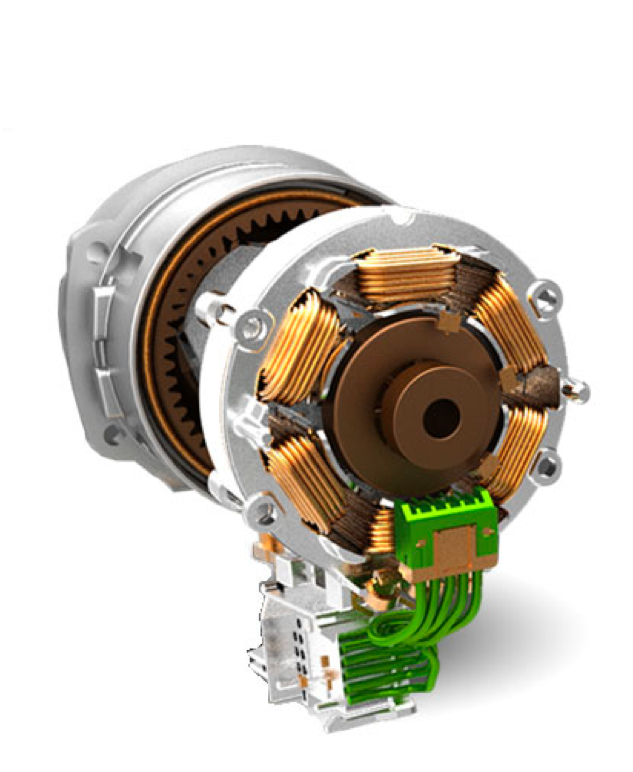
\includegraphics[width=2in]{render.png}
        \end{center}
    \end{frame}

    \begin{frame}{Overview}
        \begin{itemize}
            \item {\large Background}\\
            Brushless DC Motors
            \item {\large Theory}\\
            Magneto-statics, Permanent Magnets, Non Linear Materials, Non Linear FEM
            \item {\large Implementation}\\
            Meshing, Matrix Assembly, Solvers, BLDC Problem
            \item {\large Results}\\
            Diagrams, Torques
        \end{itemize}

    \end{frame}

    \begin{frame}{Brushless DC Motors}
        BLDC motors consist of coils surrounding a permanent magnet\newline
        \begin{figure}
            \center
            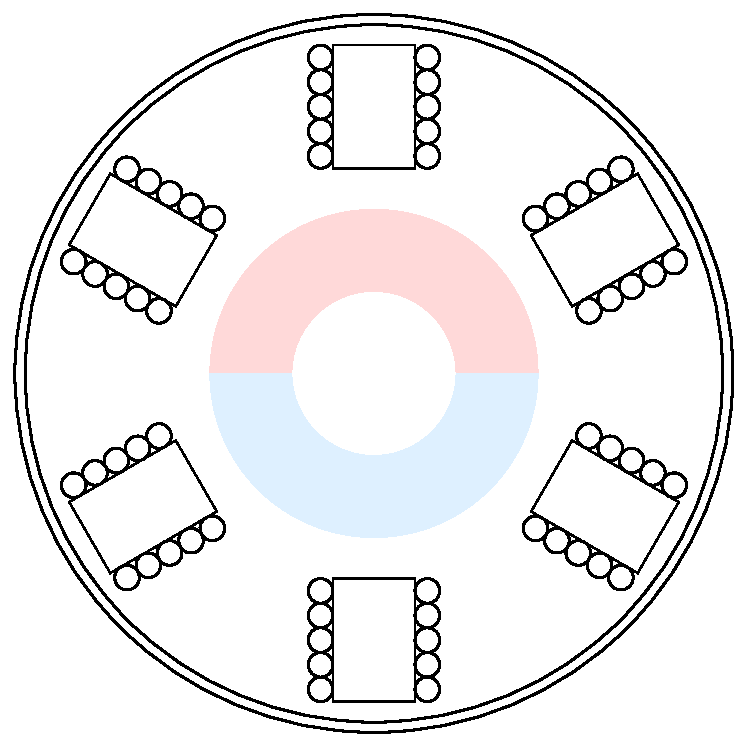
\includegraphics[width=2in]{motor_simple.pdf}
            \caption*{8 coil, 6 pole BLDC motor}
        \end{figure}
    \end{frame}

    \begin{frame}{Brushless DC Motors}
        The inner disk (rotor) is driven by the magnetic field produced by the coils
        \begin{figure}
            \center
            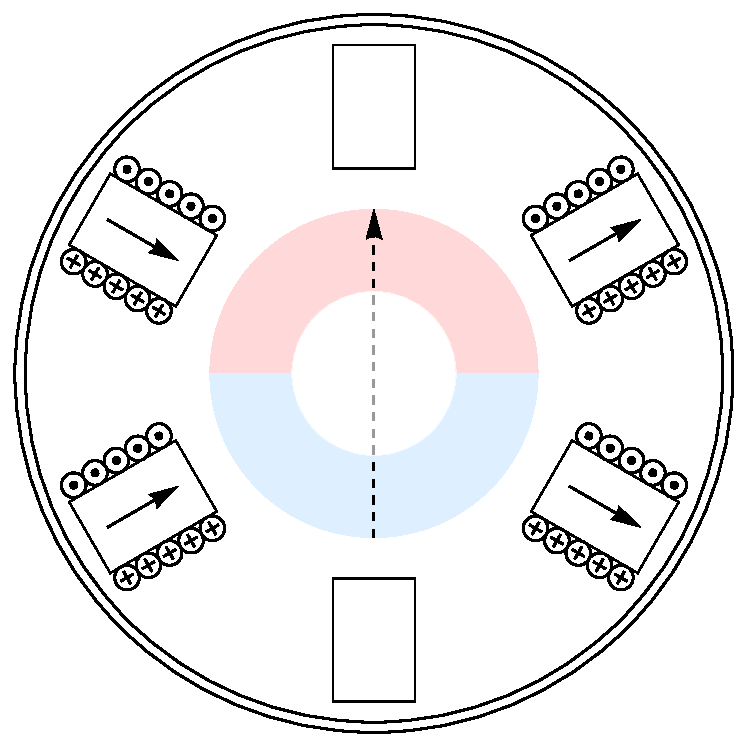
\includegraphics[width=2in]{motor_arrows.pdf}
            \caption*{Current and Magnetic Poles}
        \end{figure}
    \end{frame}

    \begin{frame}{Torque on a Magnetic Dipole}
        \[\tau = \vec{m} \times \vec{B}\]
        \begin{figure}
            \center
            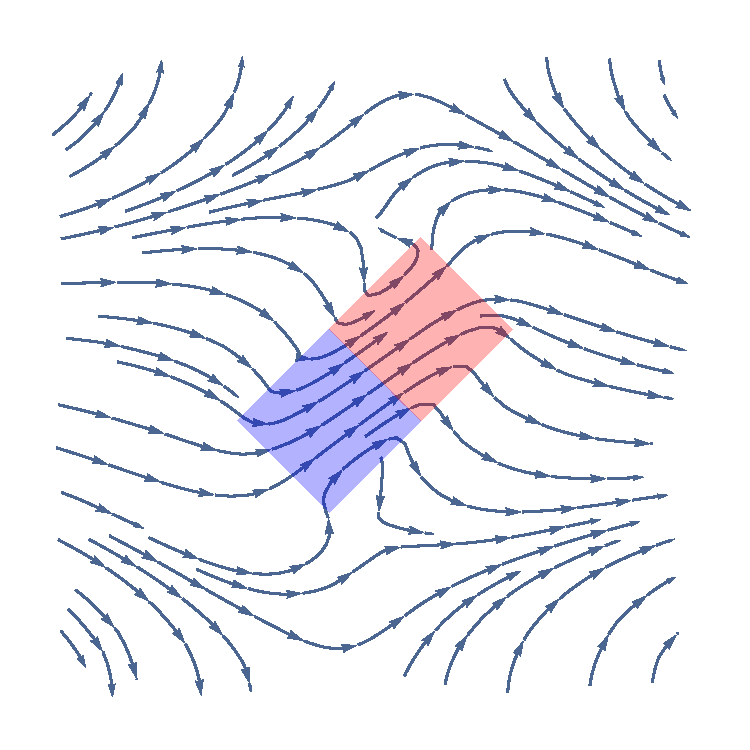
\includegraphics[width=2.5in]{Momento_torcente_magnetico.pdf}
            \caption*{Magnetic Dipole in a Uniform Field}
        \end{figure}
    \end{frame}

    \begin{frame}{Coils}
        Coils produce a field similar to that of a bar magnet
        \begin{figure}
            \center
            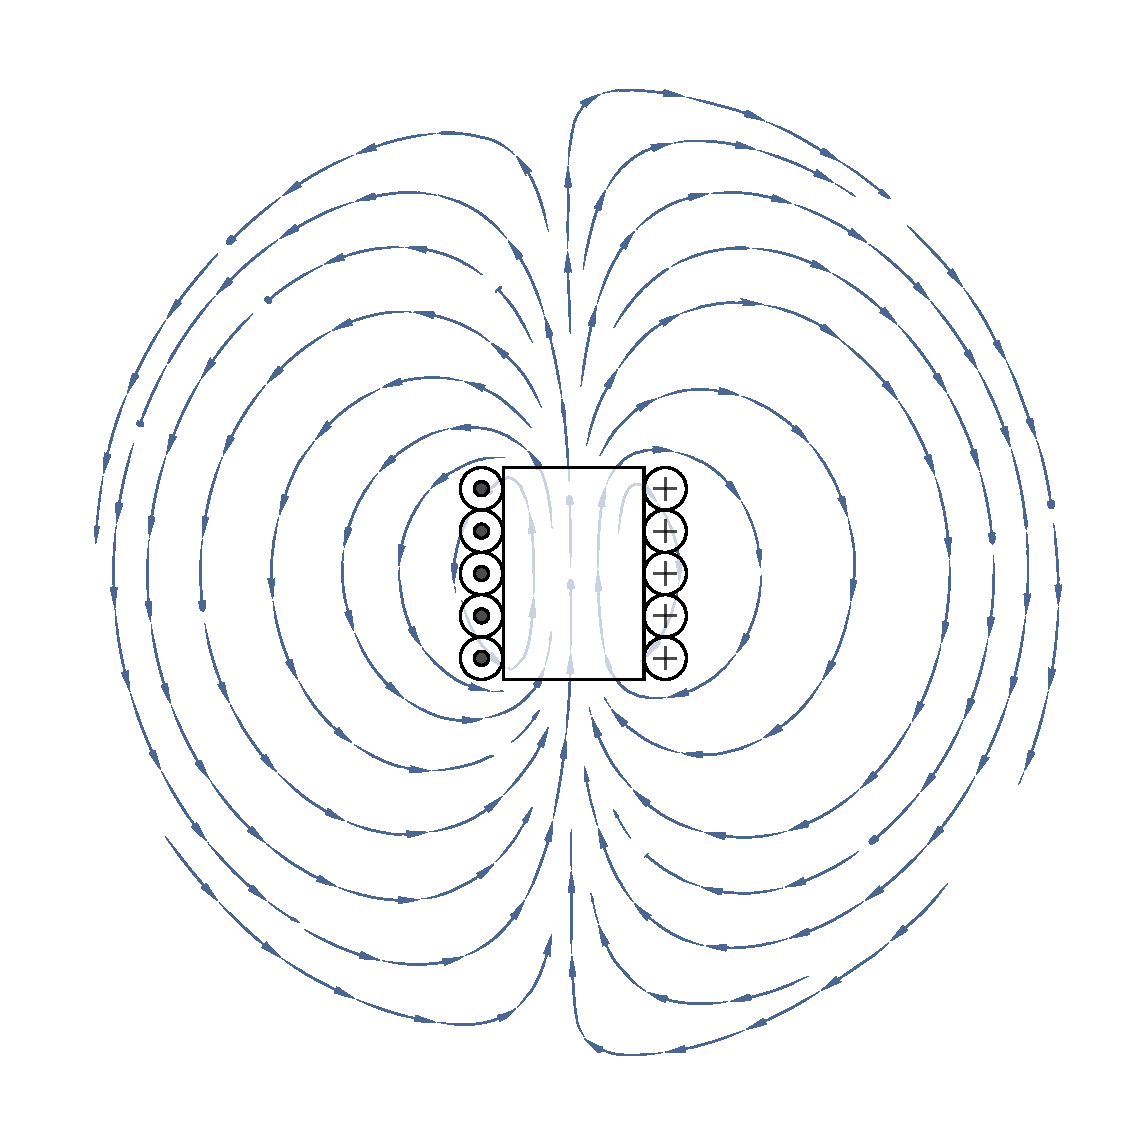
\includegraphics[width=2.5in]{coil.pdf}
            \caption*{Field produced by a motor coil}
        \end{figure}
    \end{frame}
    
    \begin{frame}{Magnetostatics in a 2D Cross Section}
        If current is only perpendicular to the 2D plane, then
        \begin{align*}
            &\nabla\times \nu B=J\text{ and }\nabla \times A = B\\
            &\nabla\times \nu \nabla\times A=J \iff \nabla\cdot \nu \nabla A=-J
        \end{align*}
        \begin{center}
            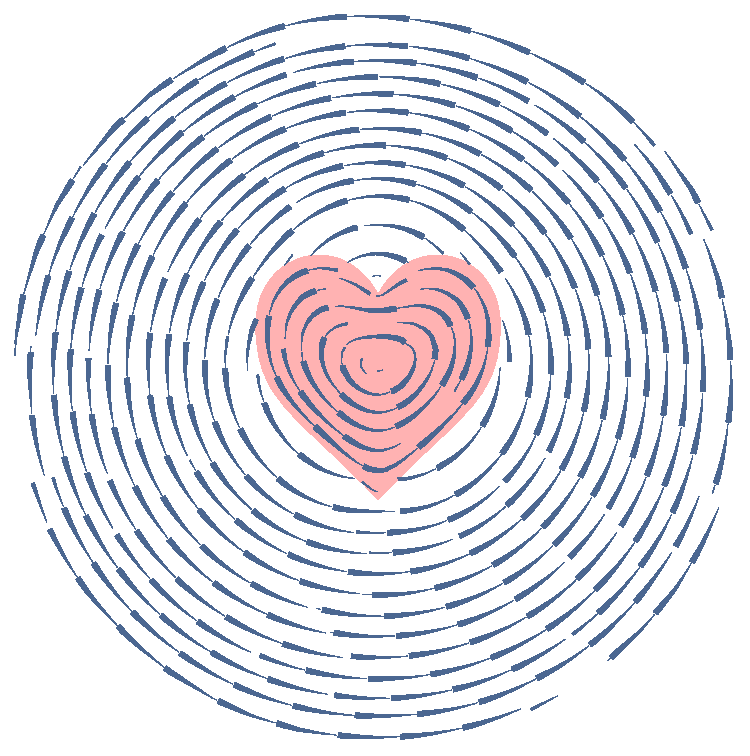
\includegraphics[width=2.5in]{heartwire.pdf}
        \end{center}
    \end{frame}
    \begin{frame}{Permanent Magnets}
        Maxwell's Equation's for Permanent Magnets
        \begin{align*}
            B &= \mu H +\mu_0 M_r\text{ and } \nabla \times H = J \implies \nabla \times \nu B=J+\nabla\times \nu\mu_0 M_r\\
            J_m&\triangleq \nabla\times \nu\mu_0 M_r \implies \nabla \times \nu B=J+J_m
        \end{align*}
        \begin{center}
            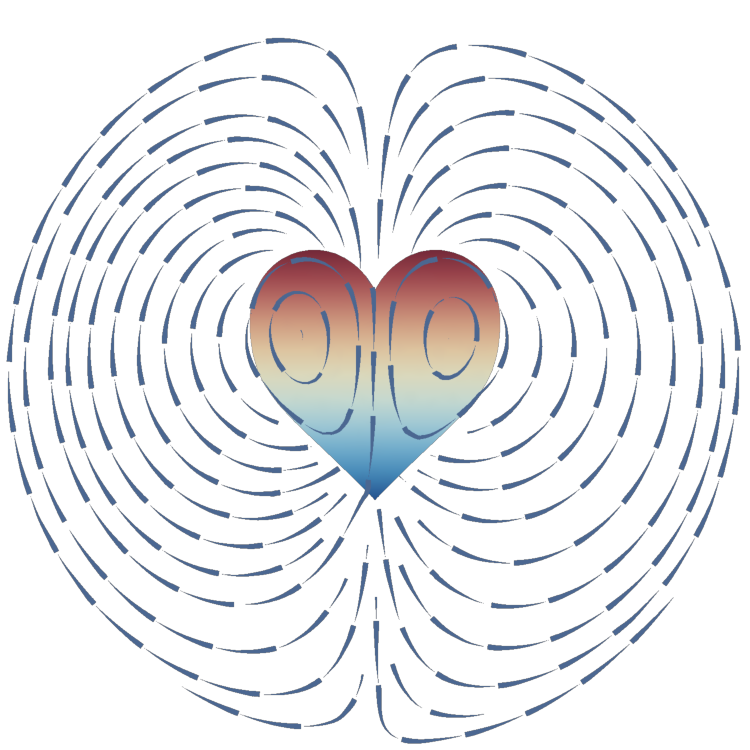
\includegraphics[width=2.5in]{heartmag.pdf}
        \end{center}
    \end{frame}
    \begin{frame}{Permenant Magnets}
        We use a \textit{2D-coil} model for permanent magnets.
        \begin{itemize}
            \item \textbf{Assumption}: A bar magnet has a similar field to a current carrying coil
            \item \textbf{Model}: Any magnet geometry can be approximated from gluing together curved bar magnets
        \end{itemize}
        \begin{figure}
            \center
            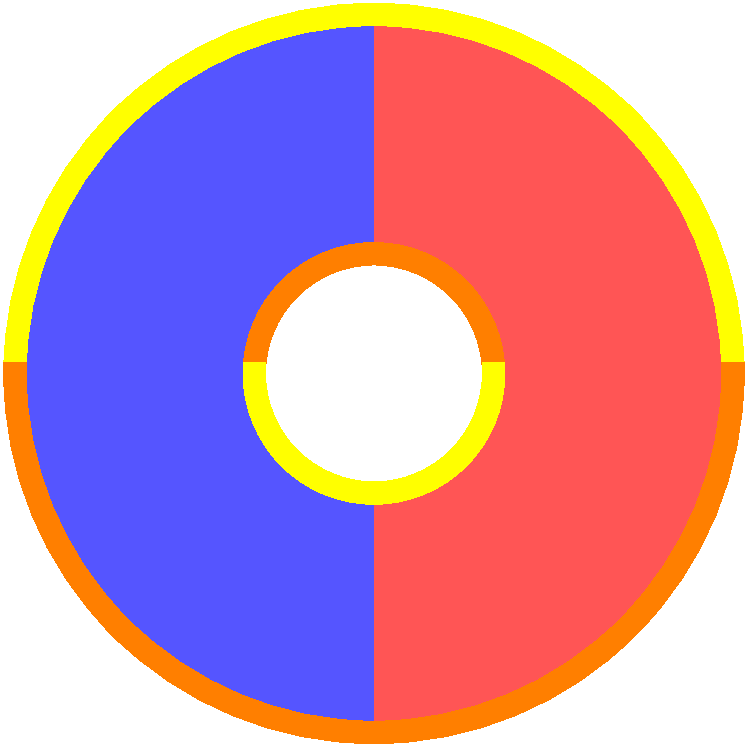
\includegraphics[width=2in]{current_magnet.pdf}
            \caption*{Yellow lines indicate current sheets coming out of the page, Orange are in}
        \end{figure}
    \end{frame}
    \begin{frame}{Permanent Magnets}
        Calculating magnetization current given a desired central field and geometry.
        \begin{gather*}
            J_m=\frac{B_c}{\int_{-L}^L \frac{\mu }{\pi  \sqrt{R^2+z^2}} \, dz}=\frac{\pi  B_c}{\mu  \log \left(\frac{2 L \left(\sqrt{L^2+R^2}+L\right)}{R^2}+1\right)}\\
            (B\to 1\text{T},L\to 5\text{cm},R\to 1\text{cm},\mu \to 1.05 \mu _0,\,J_m\approx 514814\text{A}/\text{m})\\
        \end{gather*}
        \begin{center}
            \vspace{-.5cm}
            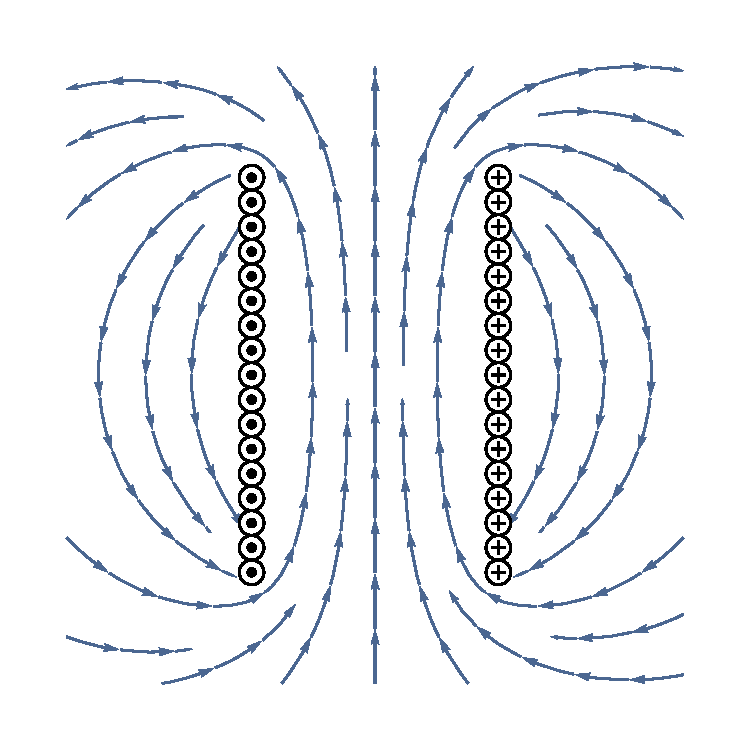
\includegraphics[width=2in]{magnet_model.pdf}
        \end{center}
    \end{frame}
    \begin{frame}{Torque}
        Force from Maxwell's Stress tensor
        \begin{gather*}
            \vec{F}=\oint_{s} \mathbf{\sigma} \cdot d S\\
            \vec{F}=\oint_{s}\left[\frac{1}{\mu_{0}}\left(B_{n} B_{t}\right) \vec{t}+\frac{1}{2 \mu_{0}}\left(B_{n}^{2}-B_{t}^{2}\right) \vec{n}\right] d S\\
        \end{gather*}
        Two dimensional simplification for the BLDC magnet
        \begin{equation*}
            \tau=\frac{1}{\mu_{0}\left(r_{s}-r_{r}\right)} \int_{r_{r}}^{r_{s}} \int_{0}^{2 \pi}\left(r^2 B_{r} B_{\theta}\right) d\theta dr
        \end{equation*}
        Since this is a two dimensional contour the output is torque per unit length
    \end{frame}
    
    \begin{frame}{BH Curves}
        A $BH$ curve is used to obtain the permeability relationship of non-linear materials in external fields.
        \begin{center}
            \hspace*{-0.7in}
            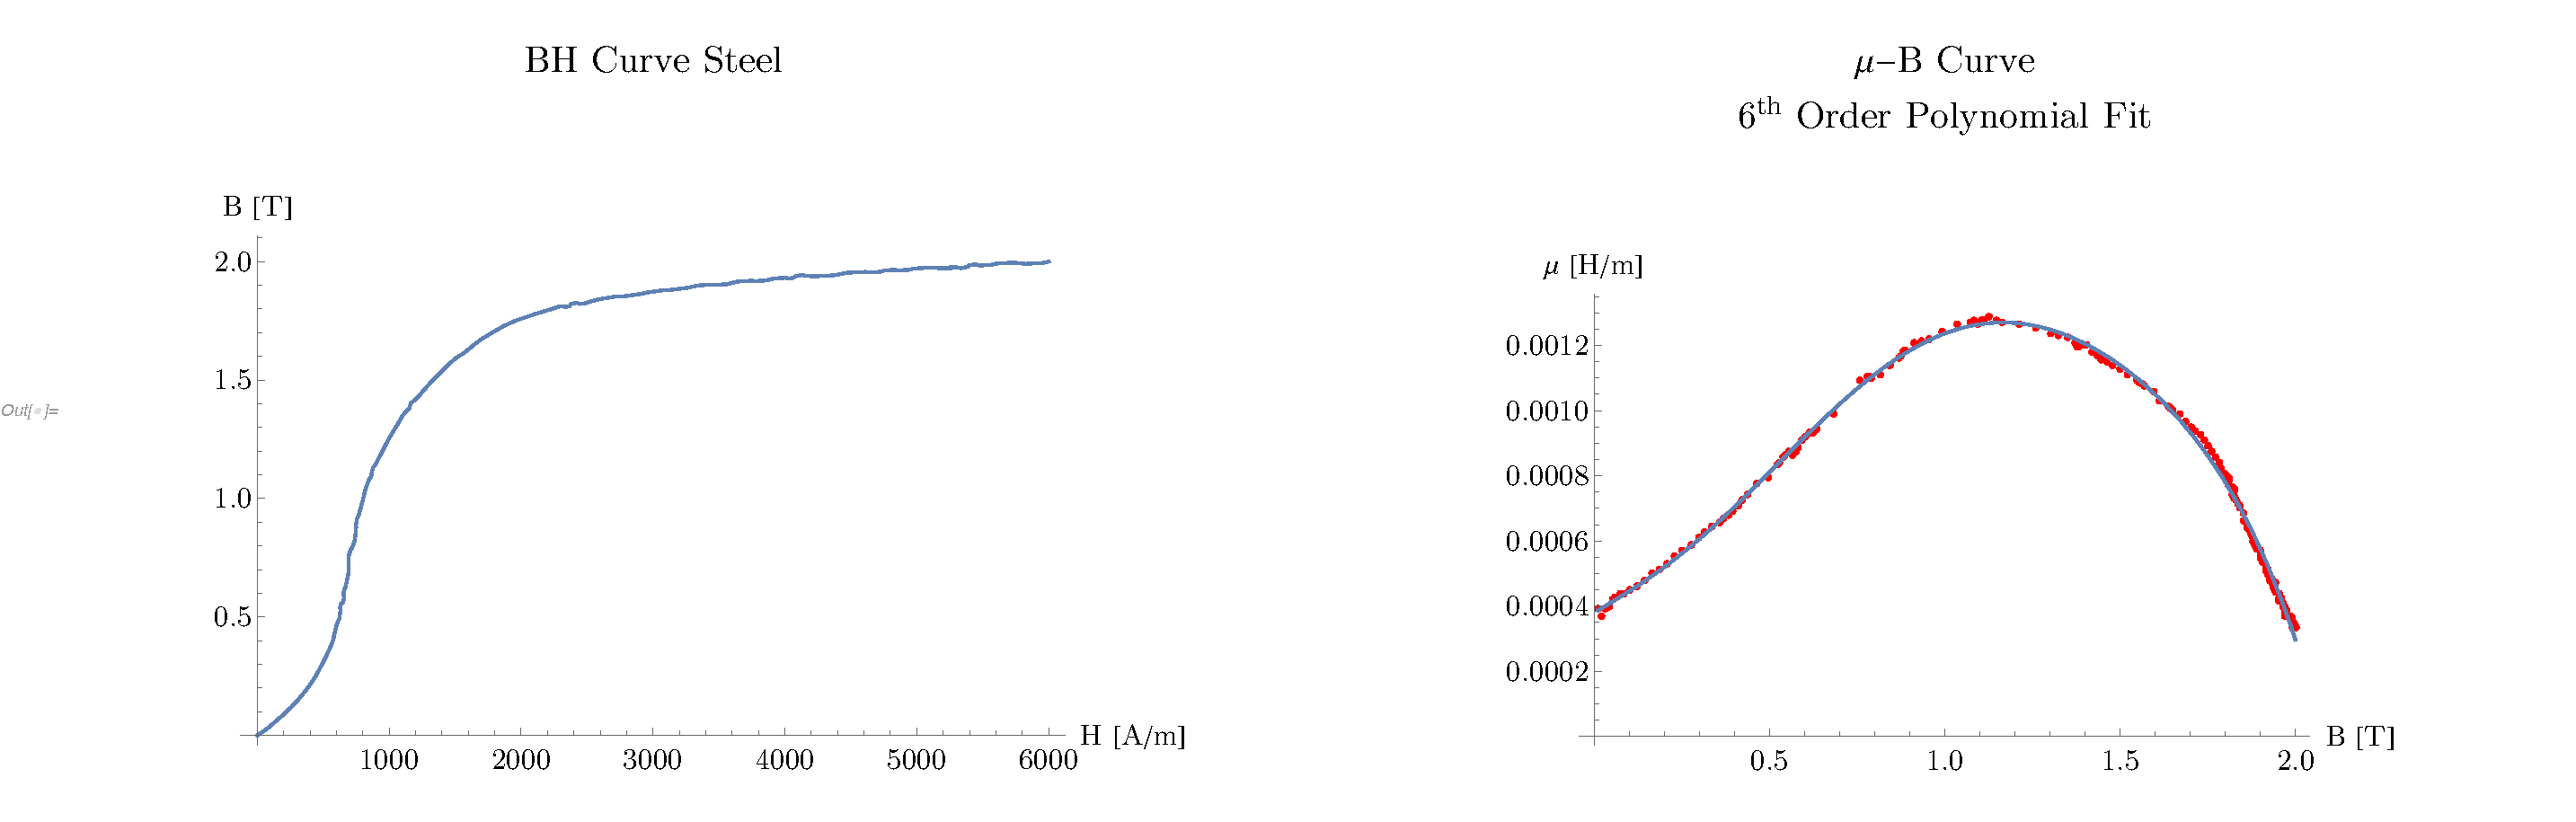
\includegraphics[width = 5.5 in]{bhcurve.pdf}
        \end{center}
        $BH$ curves for permanent magnets exhibit a hysteresis effect, however magnets have a relatively low permeability ($\mu_r\approx1.05$) and operate far from their extremes.
    \end{frame}
    
    \begin{frame}{Non Linear FEM}
        How can we use FEM to solve problems in the form of
        \[\nabla\cdot\left(\alpha(\|\nabla\phi\|)*\nabla\phi\right)=f(x,y)\]
        \textbf{First thing}: Determine $\|\nabla\phi\|$ on a single element in terms of node values of $\phi$: $\phi^{e}:=\left( \phi_i, \phi_j, \phi_k \right)^{\text{T}}$
        \begin{gather*}
            \normm{\left(\pdv{\phi}{x},\pdv{\phi}{y}\right)}=\normm{\left(\pdv{\vec{N}}{x}, \pdv{\vec{N}}{y} \right)^{\text{T}}\cdot \phi^{e}}\\
            \hat{\alpha}(\phi^e):=\alpha(\normm{\nabla\phi})
        \end{gather*}
    \end{frame}
    \begin{frame}{Solving the Non Linear System}
        Now our element matrix equation looks like:
        \[F_e(\phi^{e})=\mathbf{K}^e\cdot \phi^e*\hat{\alpha}(\phi^{e})-\vec{b}^e=0\]
        No more linear solver :( we need to use Newton's Method\\
        \smallbreak
        Consider the vector equation $f(\vec{x})=0$
        \begin{itemize}
            \item Start with the guess $\vec{x}\approx\vec{x}_0$
            \item Expand in power series
            \[f(\vec{x})\approx f(\vec{x}_0)+\mathbf{J}_{f(\vec{x}_0)}(\vec{x}-\vec{x}_0)\approx 0\]
            \item Solve a linear system for $\vec{x_0}$ to find a better guess for $\vec{x}$.
            Iterate.
            \begin{align*}
                &\mathbf{J}_{f(\vec{x}_n)}\left(\vec{x}_{n}-\vec{x}_{n+1}\right)=f(\vec{x}_{n})\\
                &\mathbf{J}_{F_e(\phi_n^e)}=\mathbf{K}^e\left( \mathbf{I}*\hat{\alpha}(\phi_n^e)+\left(\phi_n^e\right)\cdot \nabla^{\text{T}}\hat{\alpha}(\phi_n^e) \right)\\
            \end{align*}
        \end{itemize}
    \end{frame}
    \begin{frame}{Implementation: FEA\textit{lite}}
        \hspace{-0.72cm}
        
\includegraphics[width=4.5in]{technology.pdf}

    \end{frame}


    \begin{frame}{Mesh}
        \begin{itemize}
            \item Generated with Mathematica
            \item Triangular Elements
            \item Linear Shape Functions
            $A=\sum_{i=1}^{3}N_{i}A_i$
        \end{itemize}
        \begin{center}
            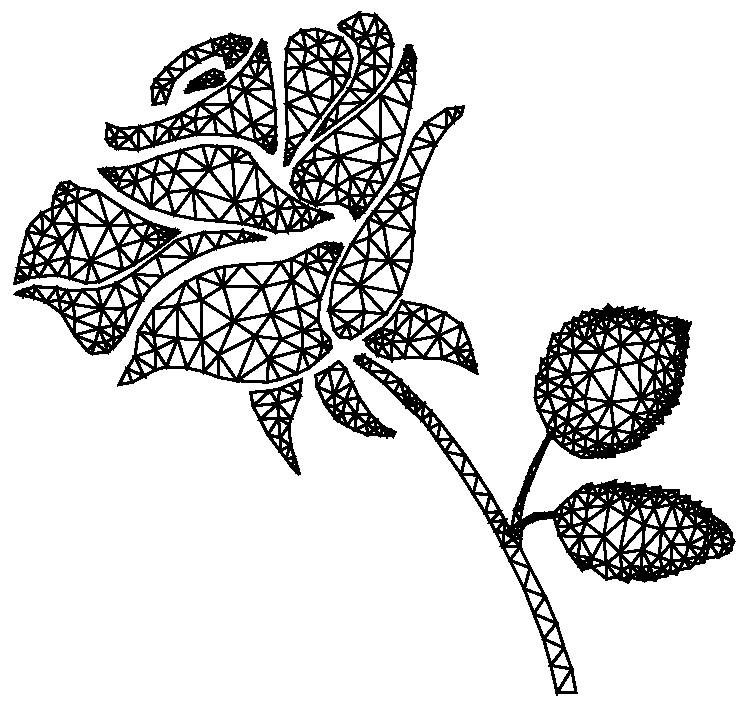
\includegraphics[width=2.8in]{rosemesh.pdf}
        \end{center}
    \end{frame}
    \begin{frame}[fragile]
        \frametitle{Matrix Assembly}
        Dense element matrices are assembled into a sparse global matrix by substituting equality constraints at shared nodes
        \[\mathbf{K}_{i,j}=\sum_{e\in E(i,j)}\sum_{k=l=0}^{3} \mathbf{K}^{e}_{k,l}*\alpha(e)\]
        $e=\{v_a,v_b,v_c\}$ is an element, $E$ is the element set, $E(i,j)$ is the set of elements $\{\,e\,|\,e\in E,\,\left(\{v_i\}\cup\{v_j\}\right)\subset e\}$, $\mathbf{K}^{e}$ is the local stiffness matrix of $e$, $\alpha$ is a function of the element properties.\\
        \begin{center}
            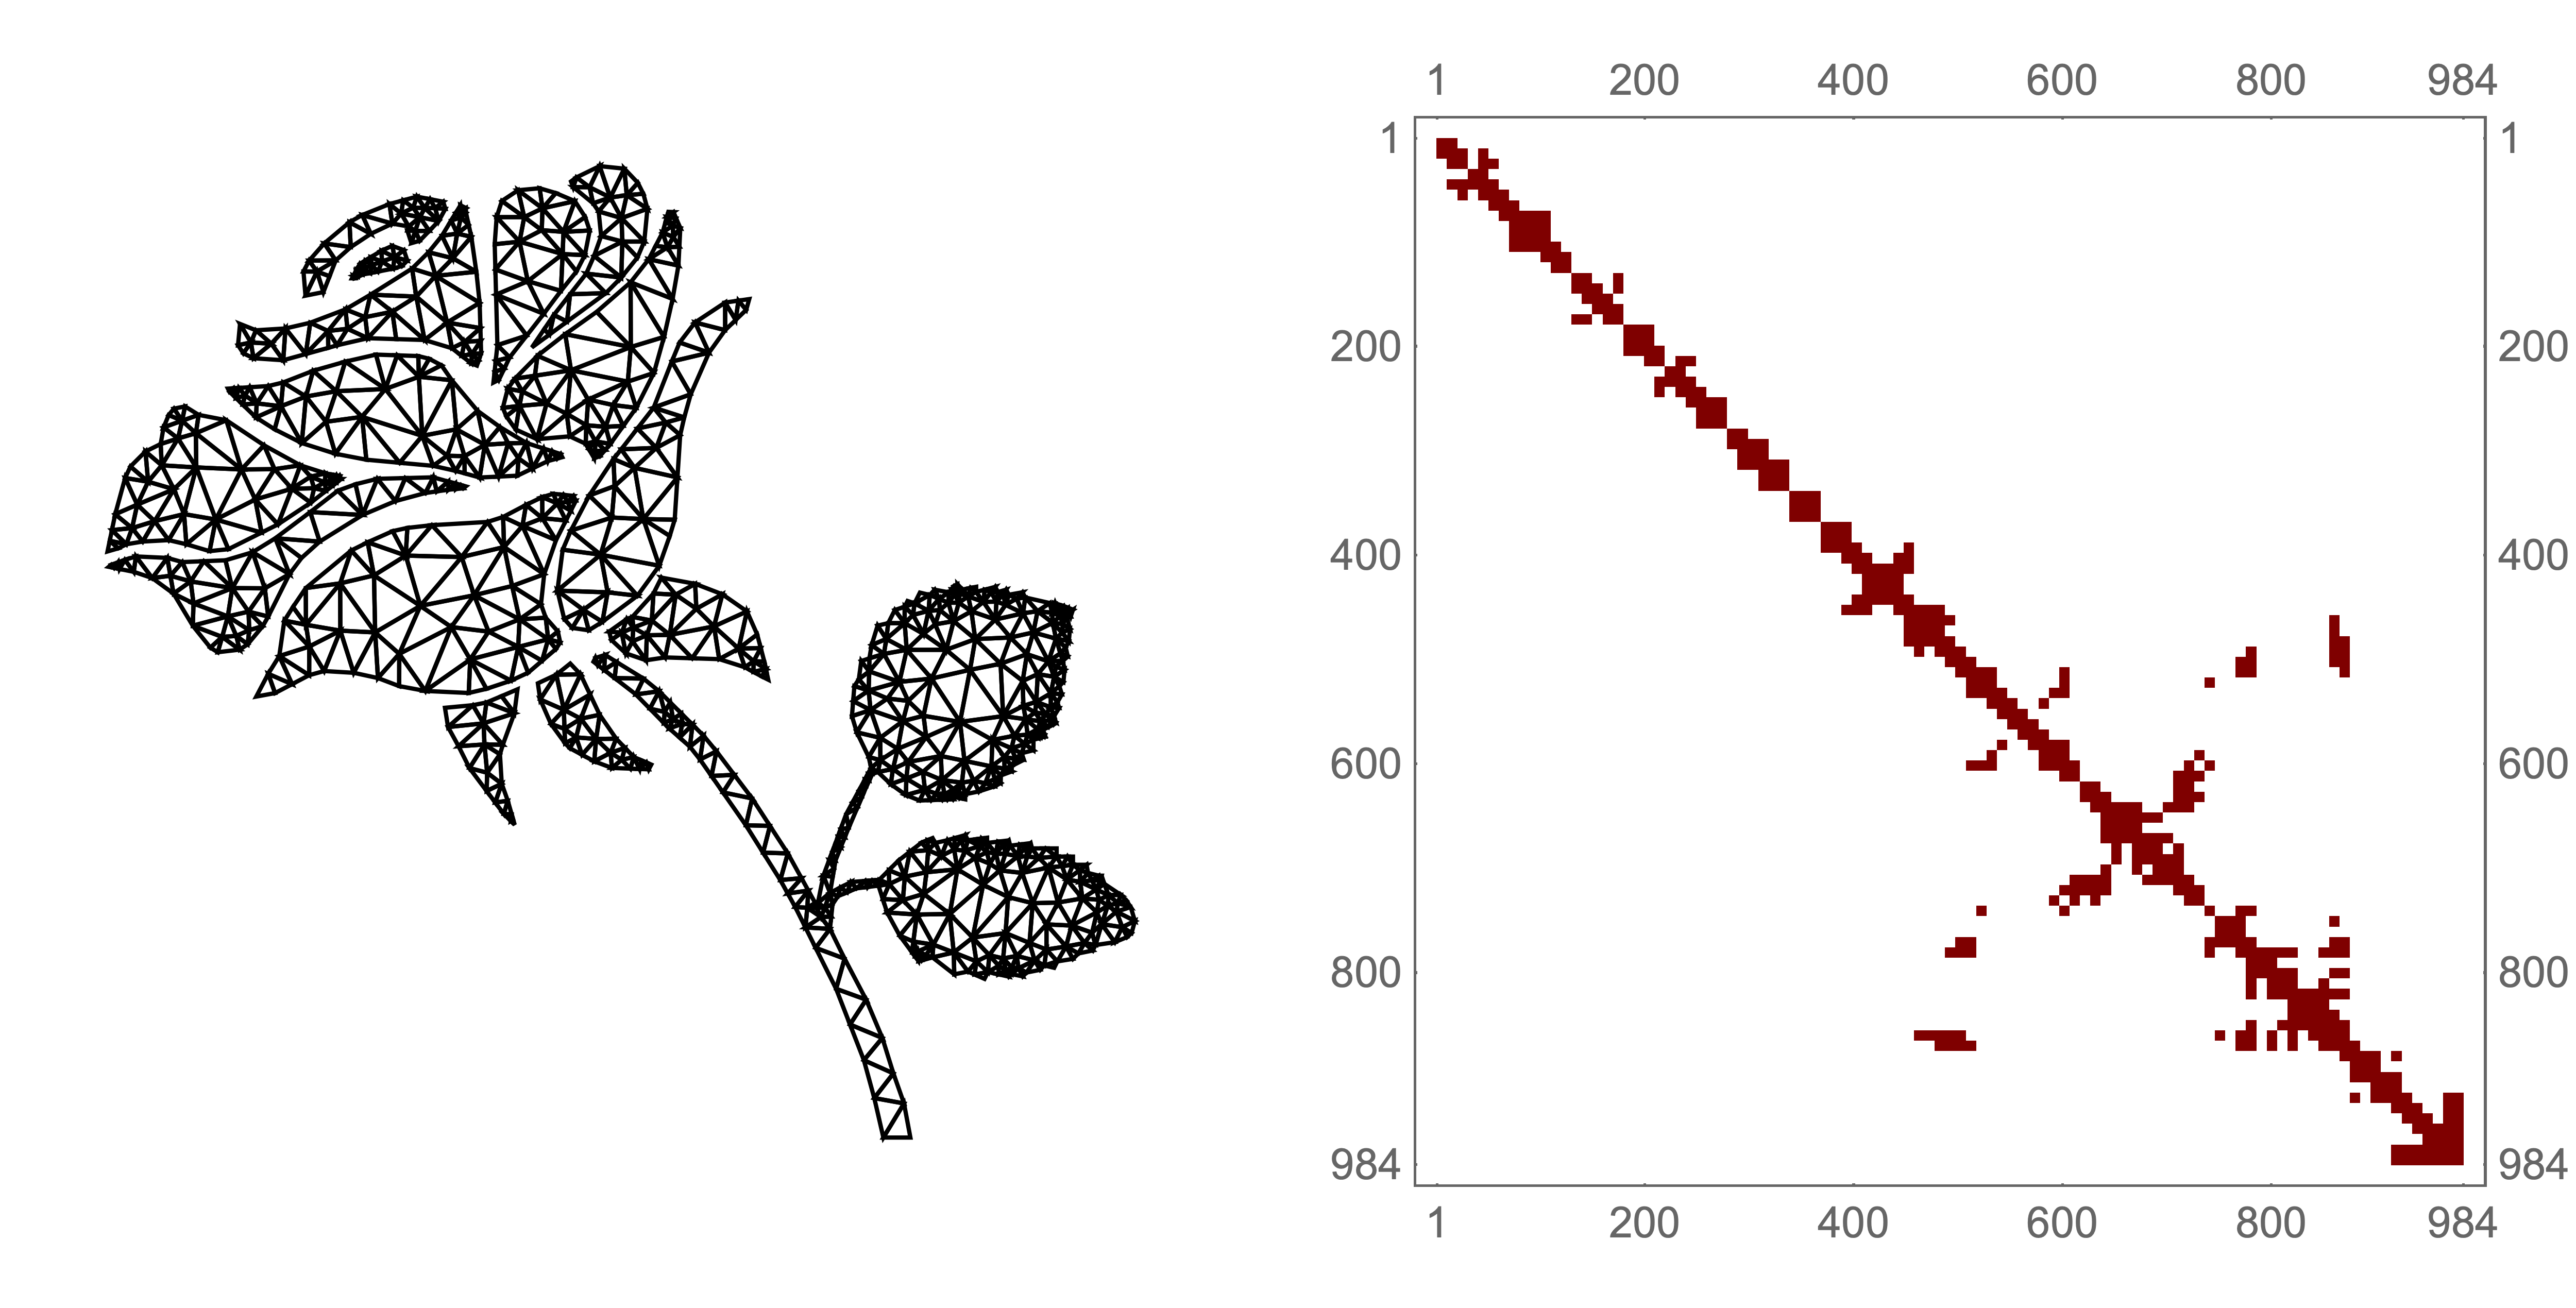
\includegraphics[width=2.5in]{meshmatrix.png}
        \end{center}
    \end{frame}

    \begin{frame}\frametitle{Solvers}
\begin{itemize}
             \item Linear FEM:\\
             Sparse linear systems solved with {\verb!scipy.linalg.sparse.spsolve}\footnote{Wrapper for SuperLU 4.0 (LU decomposition)}
            \item Non Linear FEM:
            Sparse non linear systems solved with {\verb!scipy.optimize.fsolve}\footnote{Wrapper for MINIPACK hybrj (Newton's Method + Gradient Descent)}.
            Jacobian is analytically computed to speed up the solver.
        \end{itemize}
        \begin{center}
            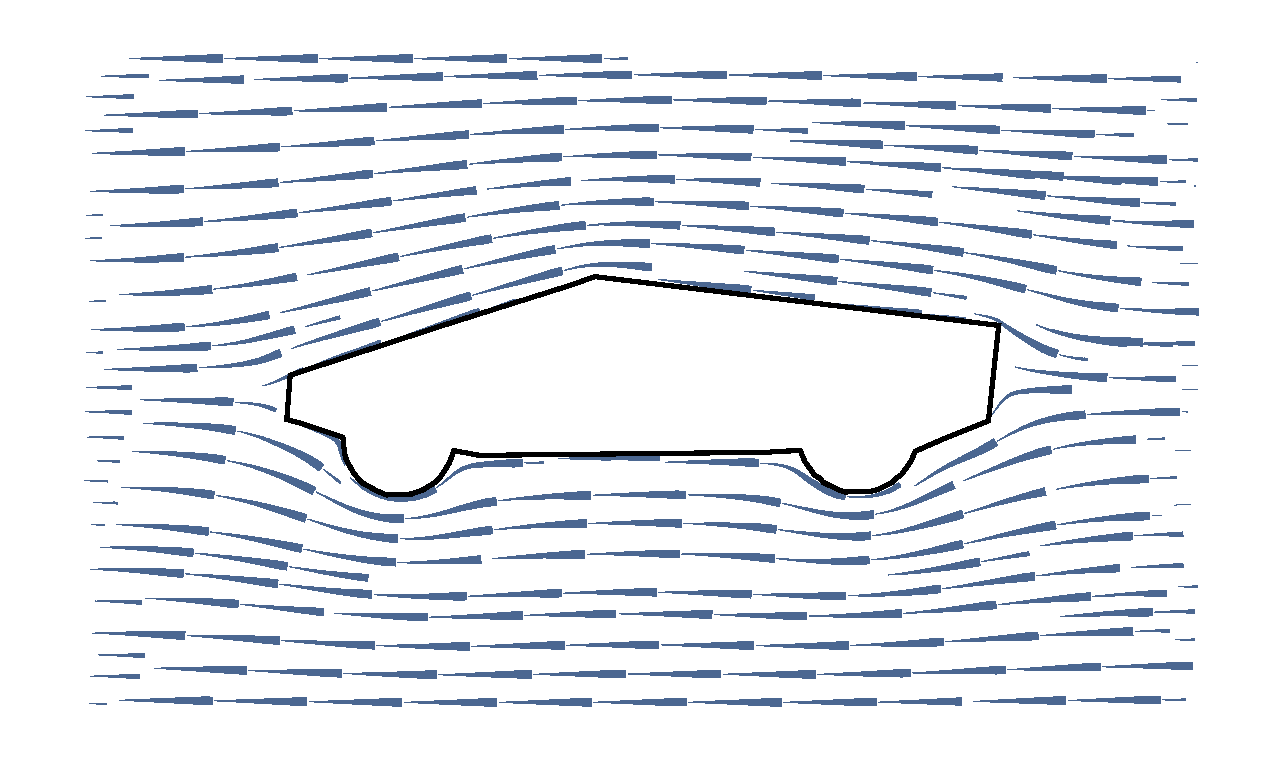
\includegraphics[width=3in]{cybercar.pdf}
        \end{center}
    \end{frame}
    \begin{frame}{BLDC Simulation}
        Mesh and Boundaries
        \begin{figure}
            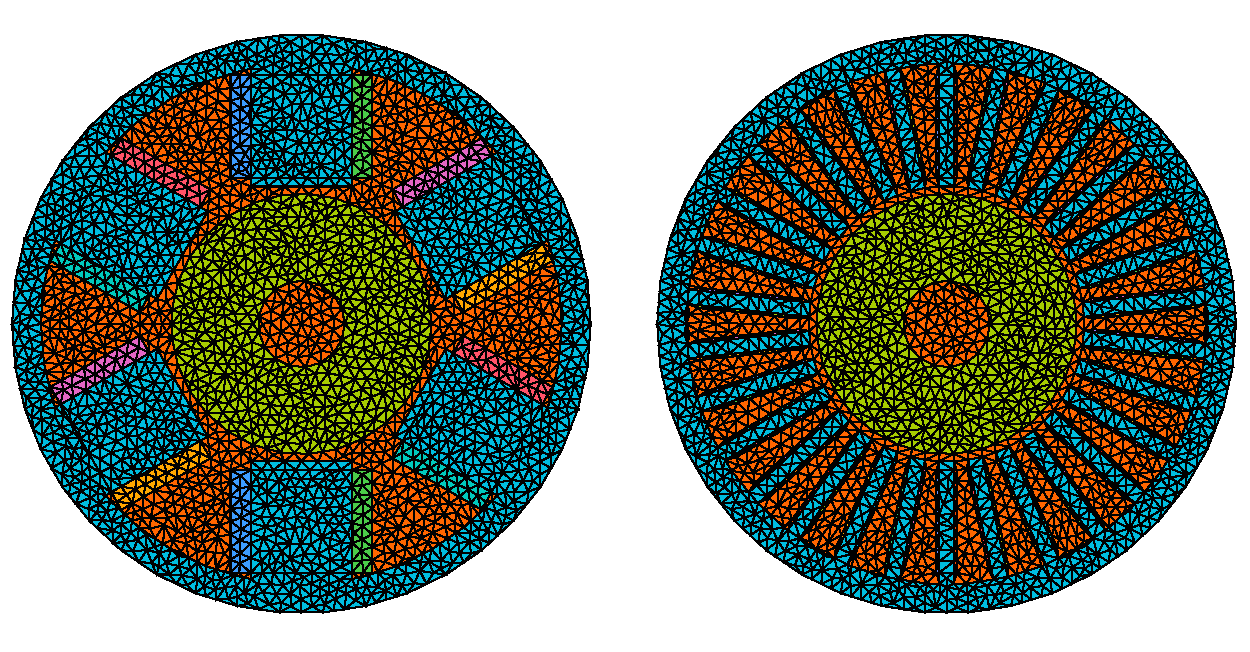
\includegraphics[width=\linewidth]{mmesh.pdf}
            \caption*{(left) 6 coils 9775 unknowns (right) 30 coils 10843 unknowns}
        \end{figure}
    \end{frame}
    \begin{frame}{BLDC Simulation}
        No Current
        \begin{figure}
            \centering
            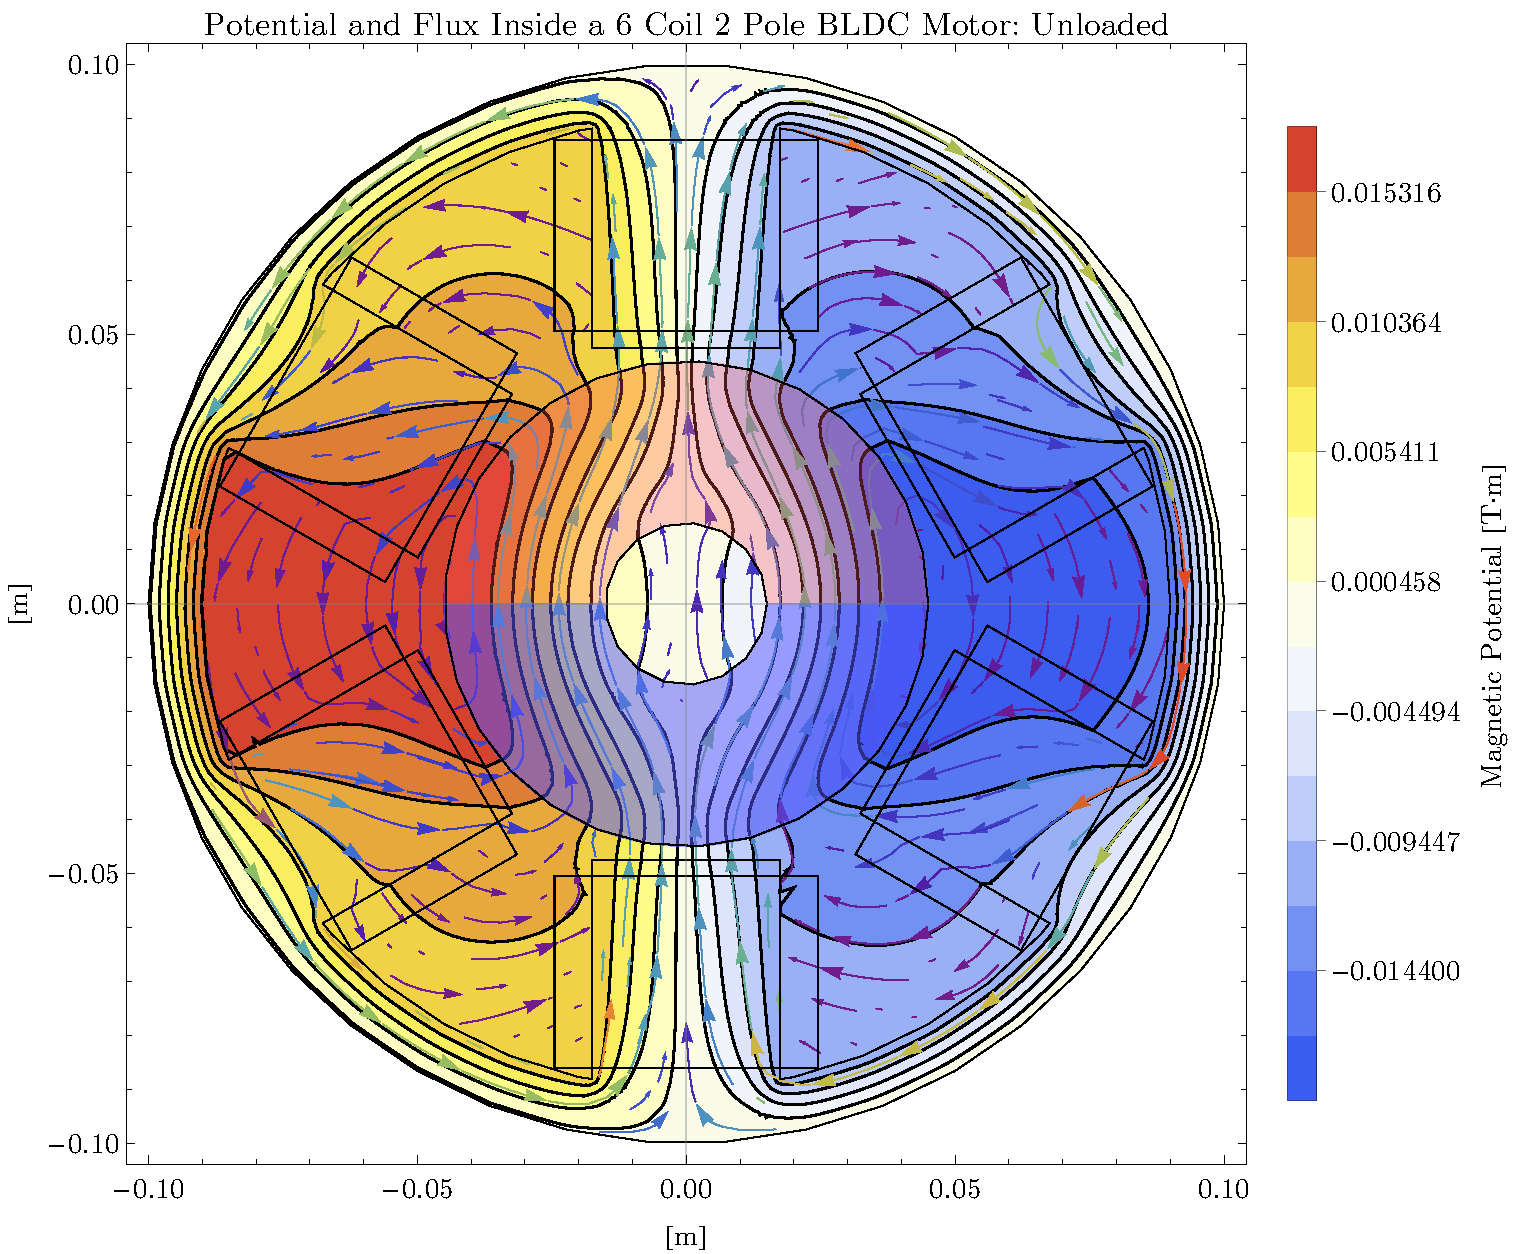
\includegraphics[width=3in]{potential-unloaded-6coils.pdf}
            \label{fig:my_label}
        \end{figure}
    \end{frame}
    
    \begin{frame}{BLDC Simulation}
        No Current
        \begin{figure}
            \centering
            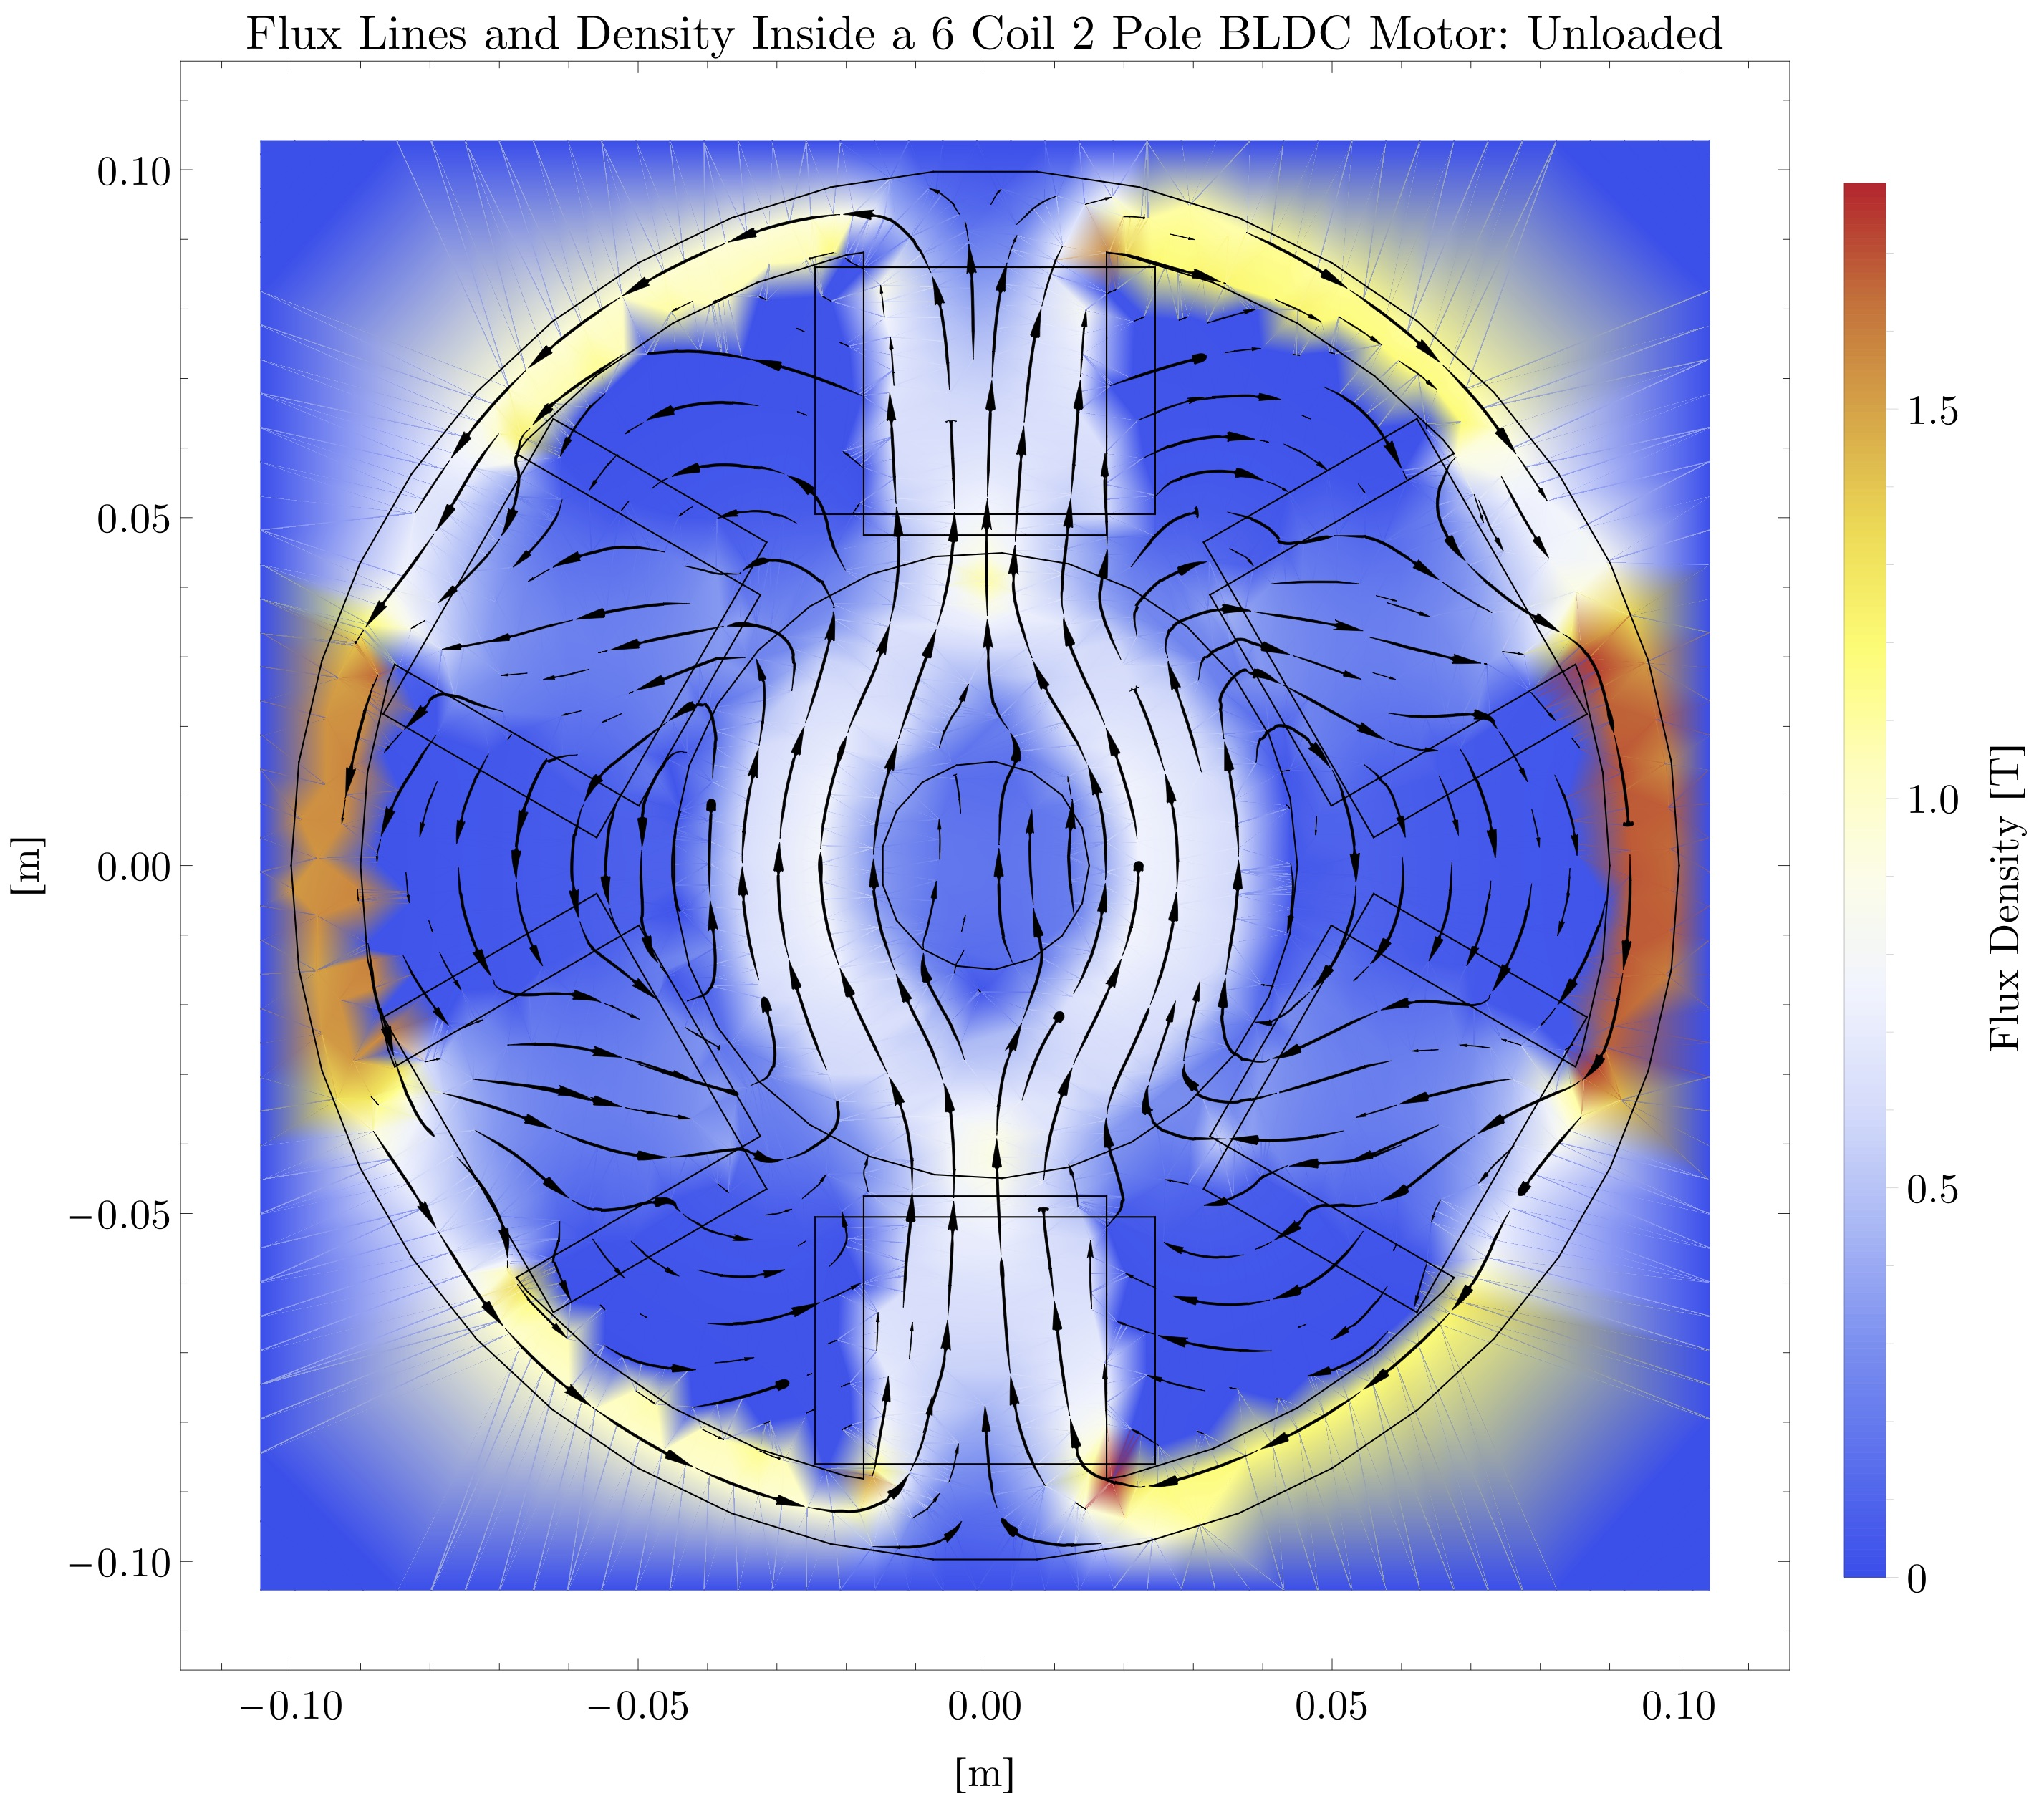
\includegraphics[width=3in]{flux-unloaded-6coils.jpg}
            \label{fig:my_label}
        \end{figure}
    \end{frame}
    
    \begin{frame}{BLDC Simulation}
        Torque
        \begin{figure}
            \centering
            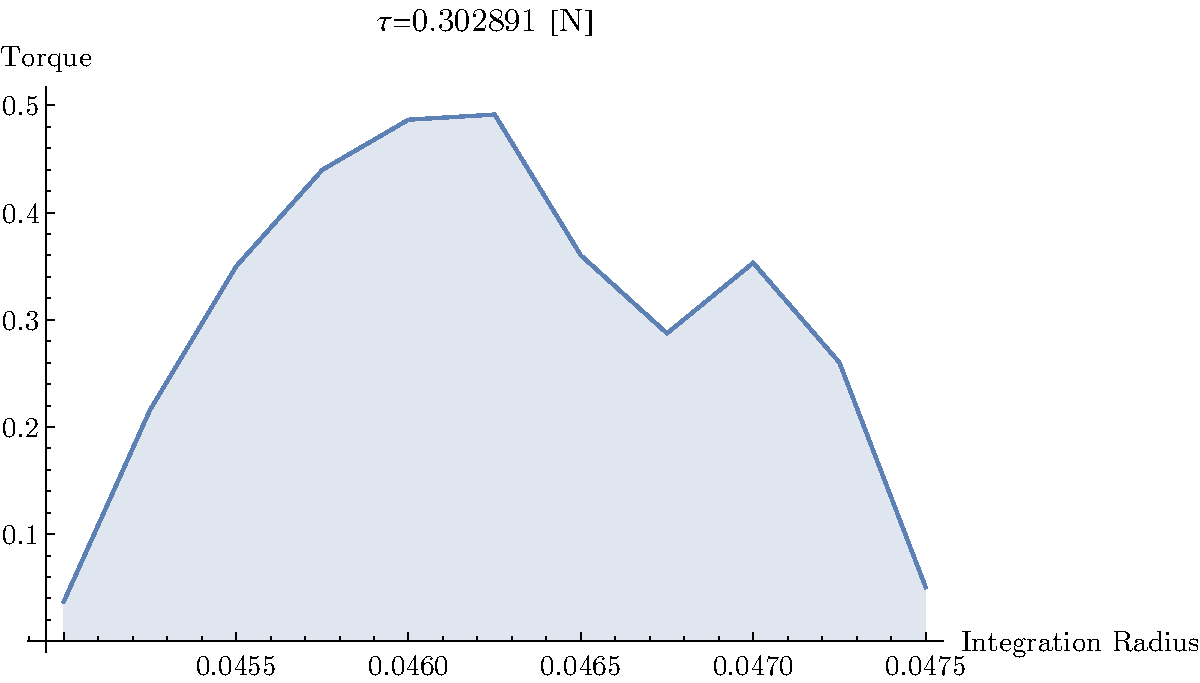
\includegraphics[width=3in]{torque-unloaded.pdf}
            \label{fig:my_label}
        \end{figure}
    \end{frame}
    
    \begin{frame}{BLDC Simulation}
        20A Load Current
        \begin{figure}
            \centering
            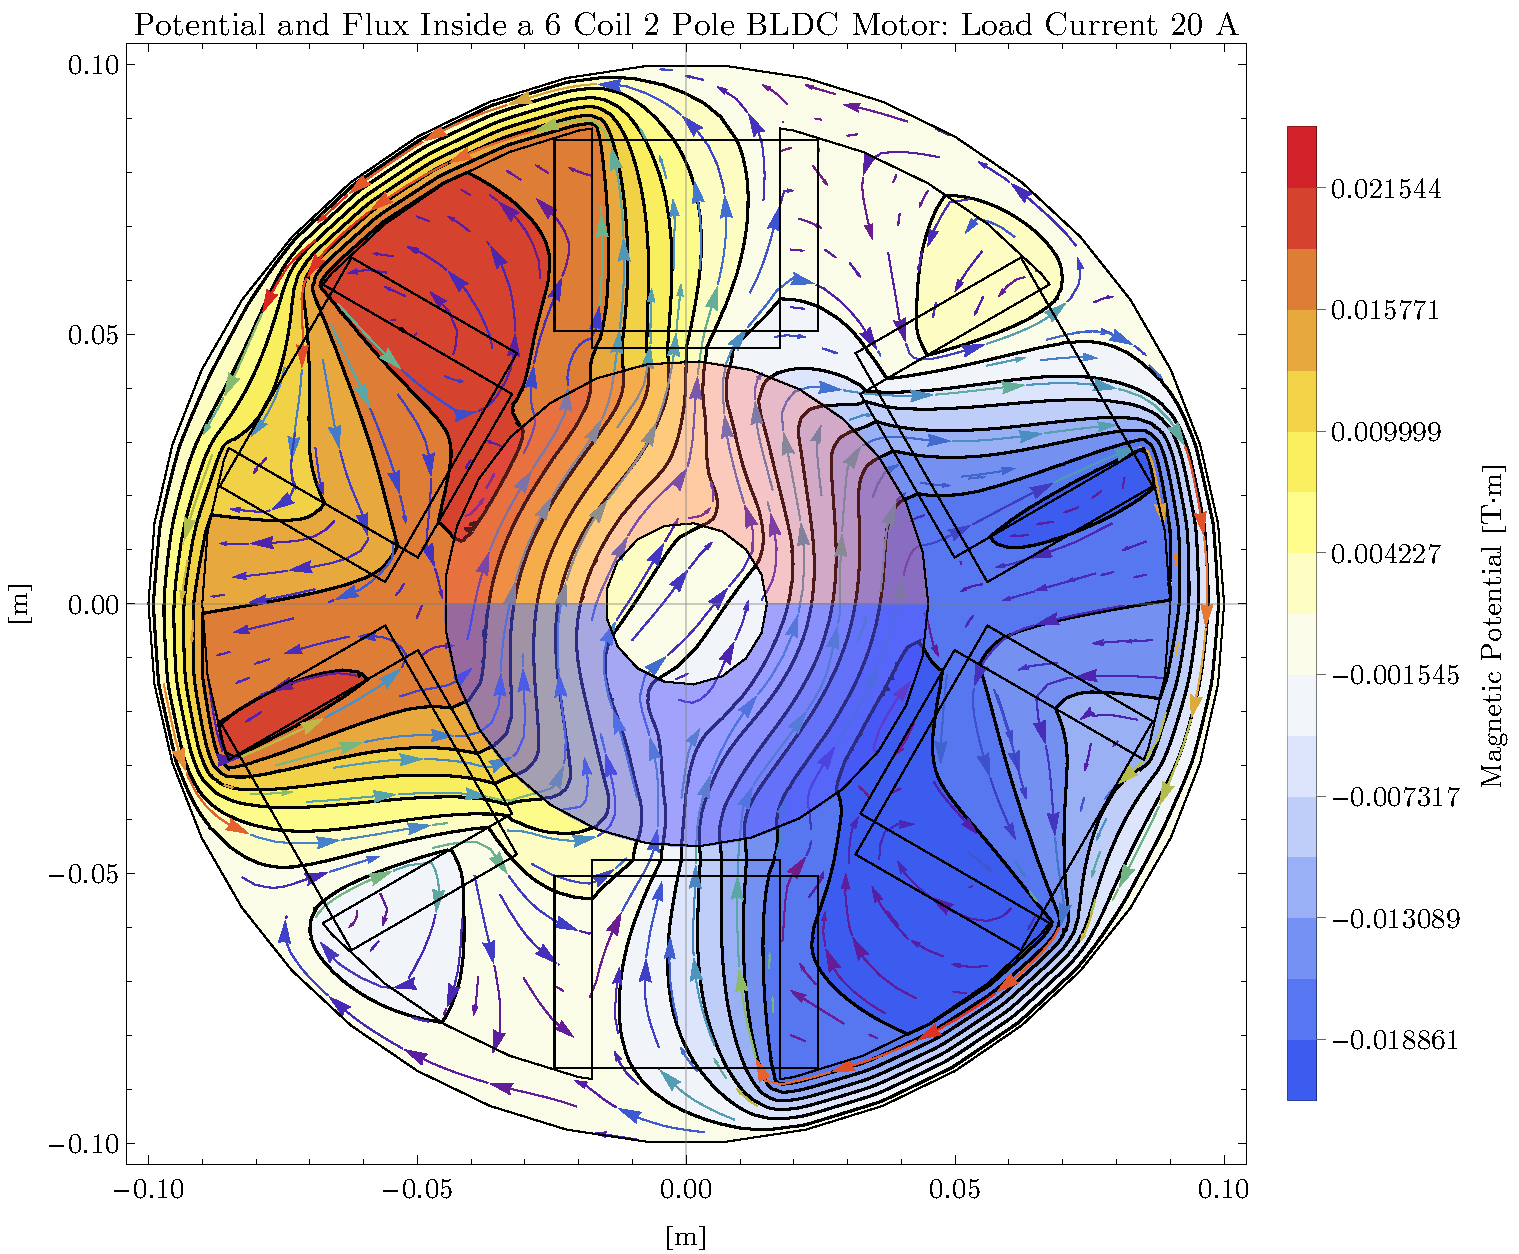
\includegraphics[width=3in]{potential-loaded-6coils.pdf}
            \label{fig:my_label}
        \end{figure}
    \end{frame}
    
    \begin{frame}{BLDC Simulation}
        20A Load Current
        \begin{figure}
            \centering
            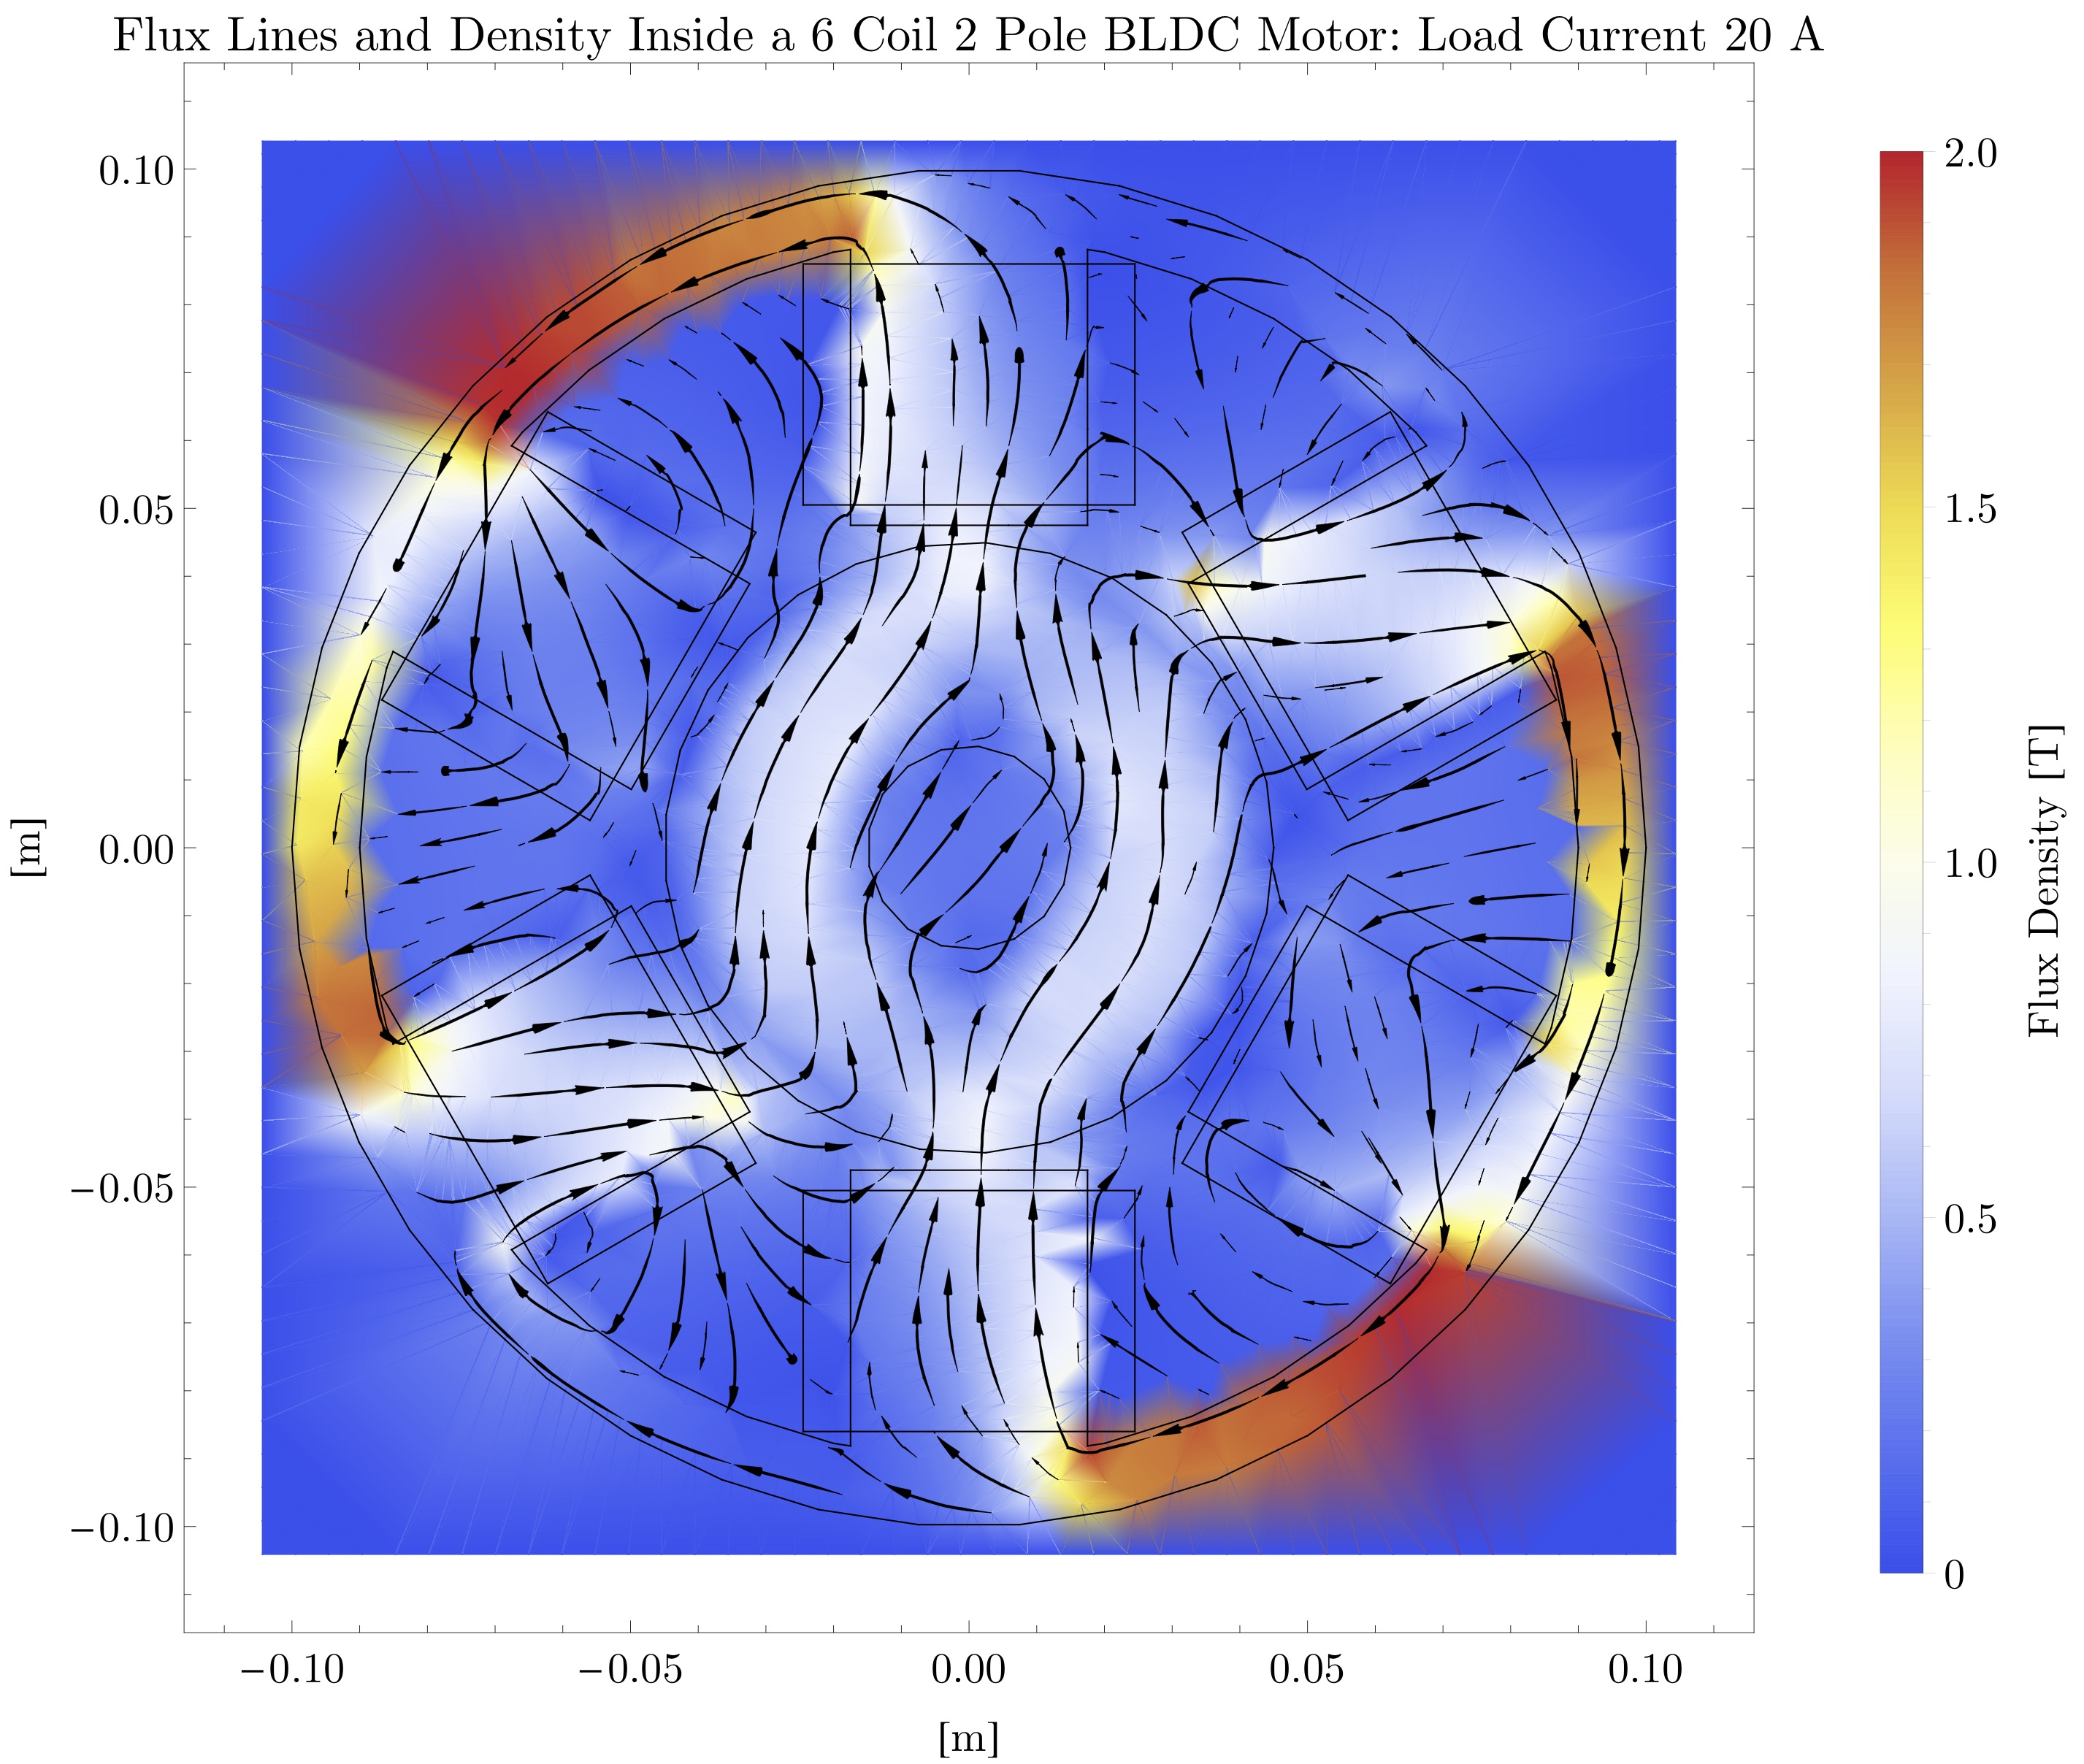
\includegraphics[width=3in]{flux-loaded-6coils.jpg}
            \label{fig:my_label}
        \end{figure}
    \end{frame}
    
    \begin{frame}{BLDC Simulation}
        Torque 
        \begin{figure}
            \centering
            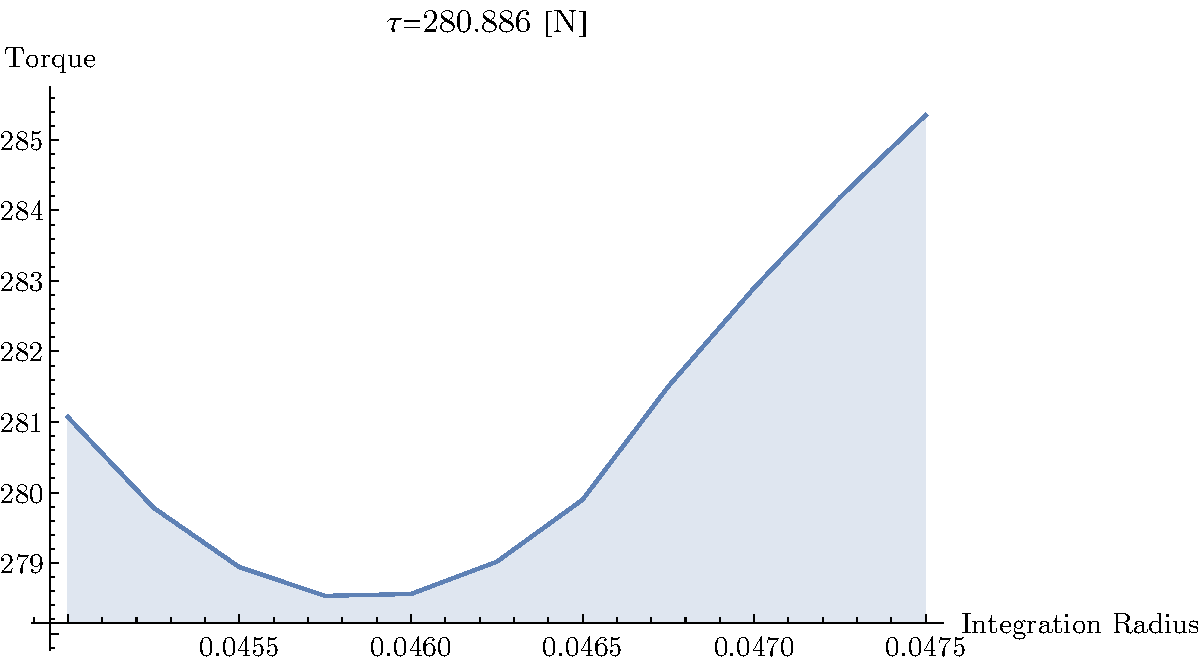
\includegraphics[width=3in]{torque1.pdf}
            \label{fig:my_label}
        \end{figure}
    \end{frame}
    
    \begin{frame}{BLDC Simulation}
        Rotated Magnet
        \begin{figure}
            \centering
            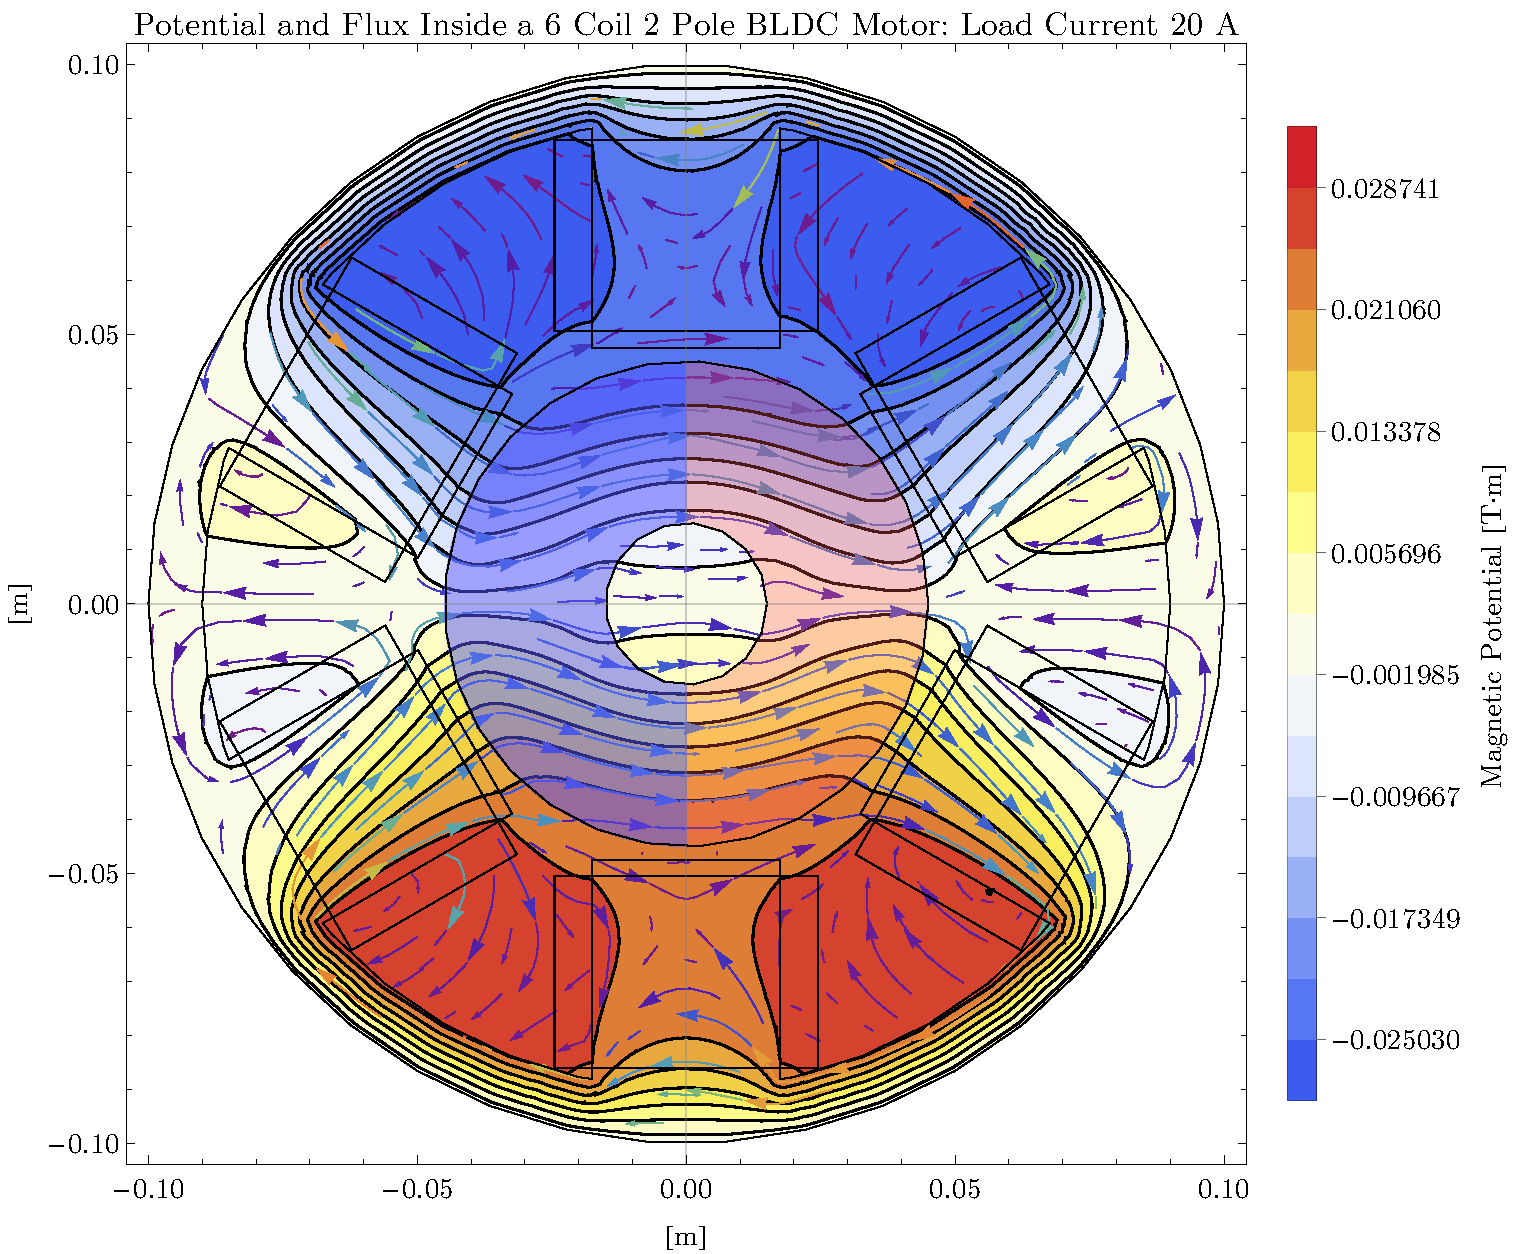
\includegraphics[width=3in]{potential-rot90-6coils.pdf}
            \label{fig:my_label}
        \end{figure}
        As hoped $\tau \approx 0$ [N]
    \end{frame}
    
    \begin{frame}{BLDC Simulation}
        More Coils and Poles
        \begin{figure}
            \centering
            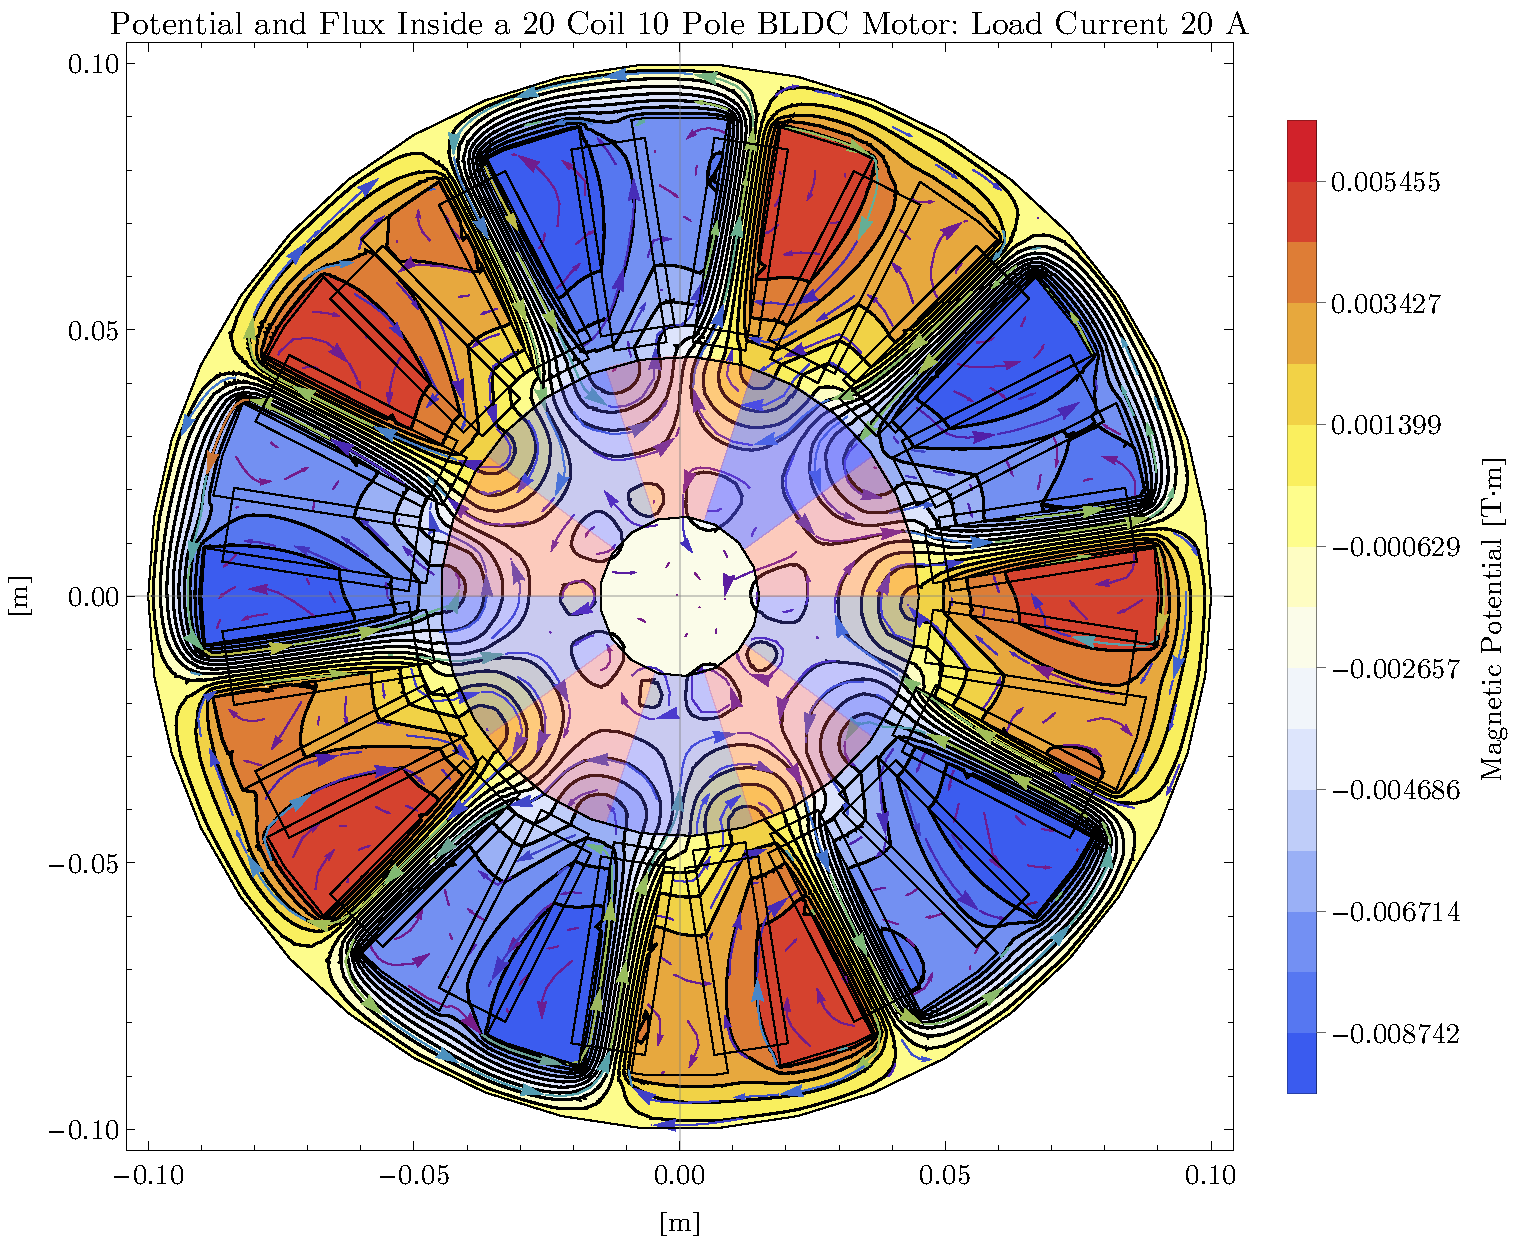
\includegraphics[width=3in]{potential-loaded-20coils.pdf}
            \label{fig:my_label}
        \end{figure}
        $\tau\approx 250$ [N]
    \end{frame}
    
    \begin{frame}{BLDC Simulation}
        More Coils and Poles
        \begin{figure}
            \centering
            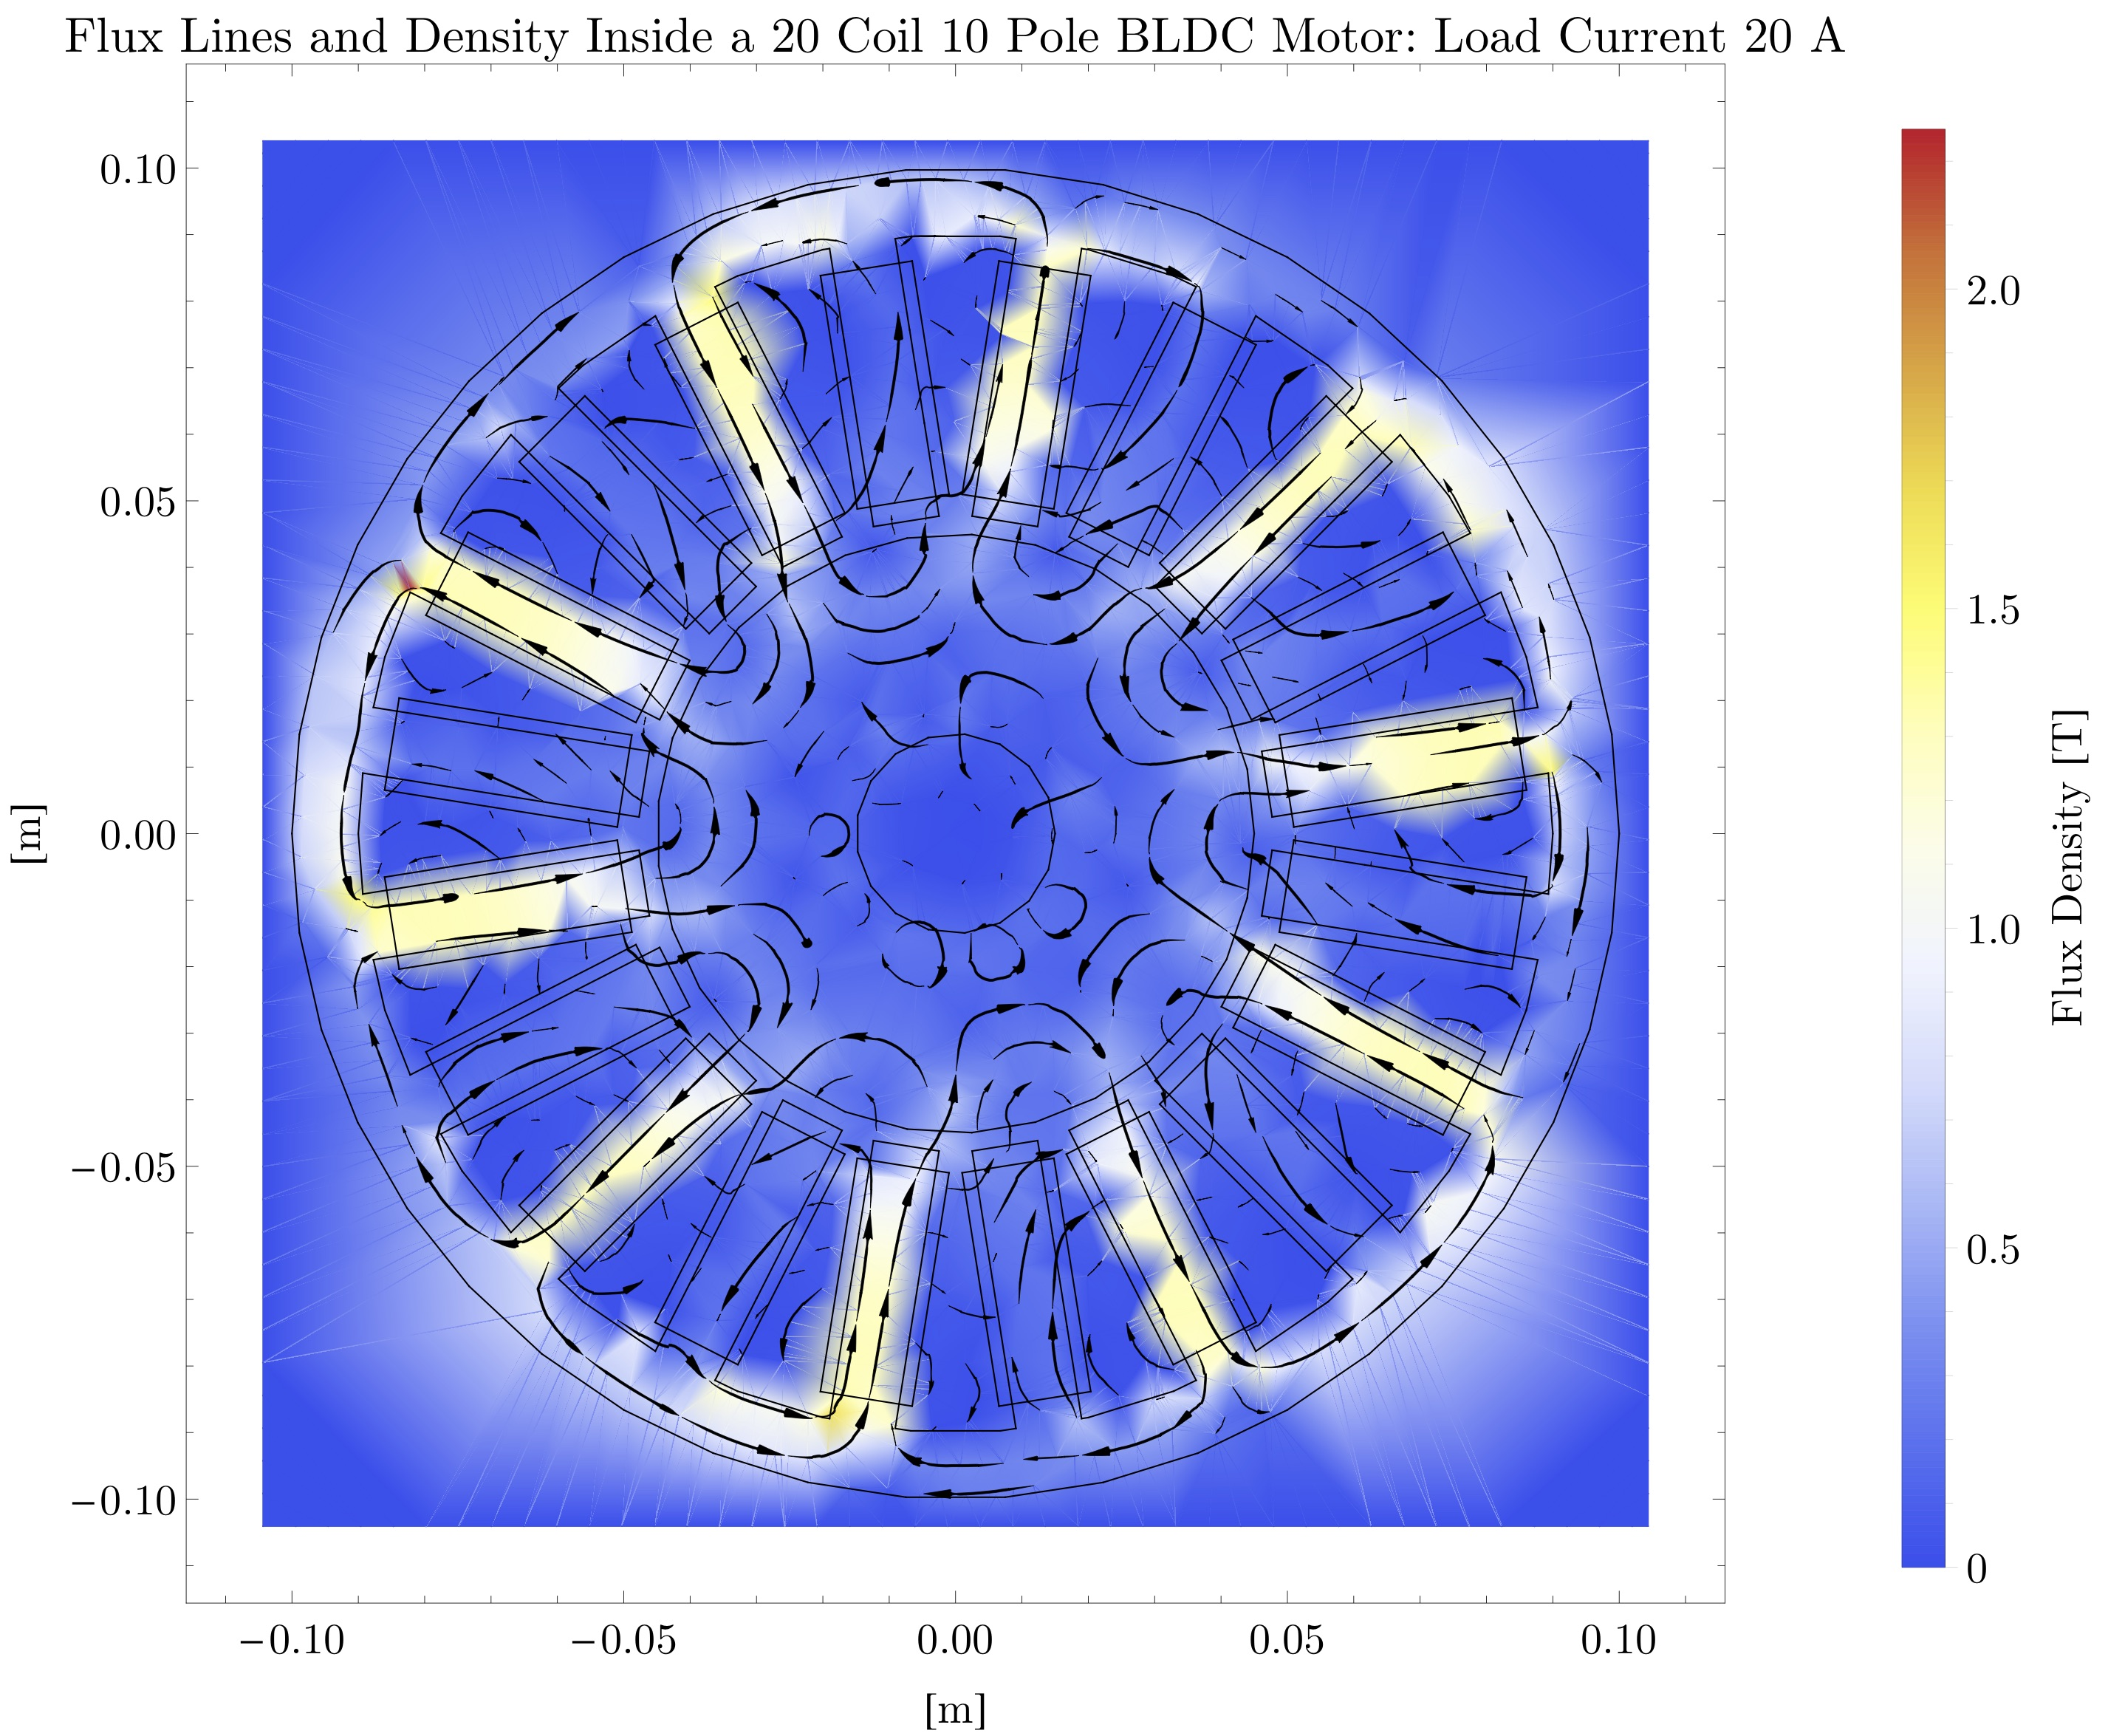
\includegraphics[width=3in]{flux-loaded-20coils.jpg}
            \label{fig:my_label}
        \end{figure}
    \end{frame}
    
        \begin{frame}{Appendix: Coil Values}
    
        Assumptions:
        \begin{itemize}
            \item Wire diameter = 1mm
            \item Current = 20A
        \end{itemize}
        \hspace{5pt} This results in a current density of:
        
        $$\frac{20A}{\frac{\pi}{4} * 1mm^2} = 25.5 \  \frac{MA}{m^2}$$
        
    \end{frame}
    
    \begin{frame}{Appendix: Mesh Generation and Format}
        \begin{itemize}
            \item Meshes are generated using the Mathematica 12 mesh generator
            \item Exported as:\\ list of coordinates [$x$, $y$]$^v$ \\list of mesh elements [$v_1$, $v_2$, $v_3$, marker]$^{e}$ \\list of boundary elements [$v_1$, $v_2$, marker]$^{be}$
        \end{itemize}


        \begin{figure}
            \centering
            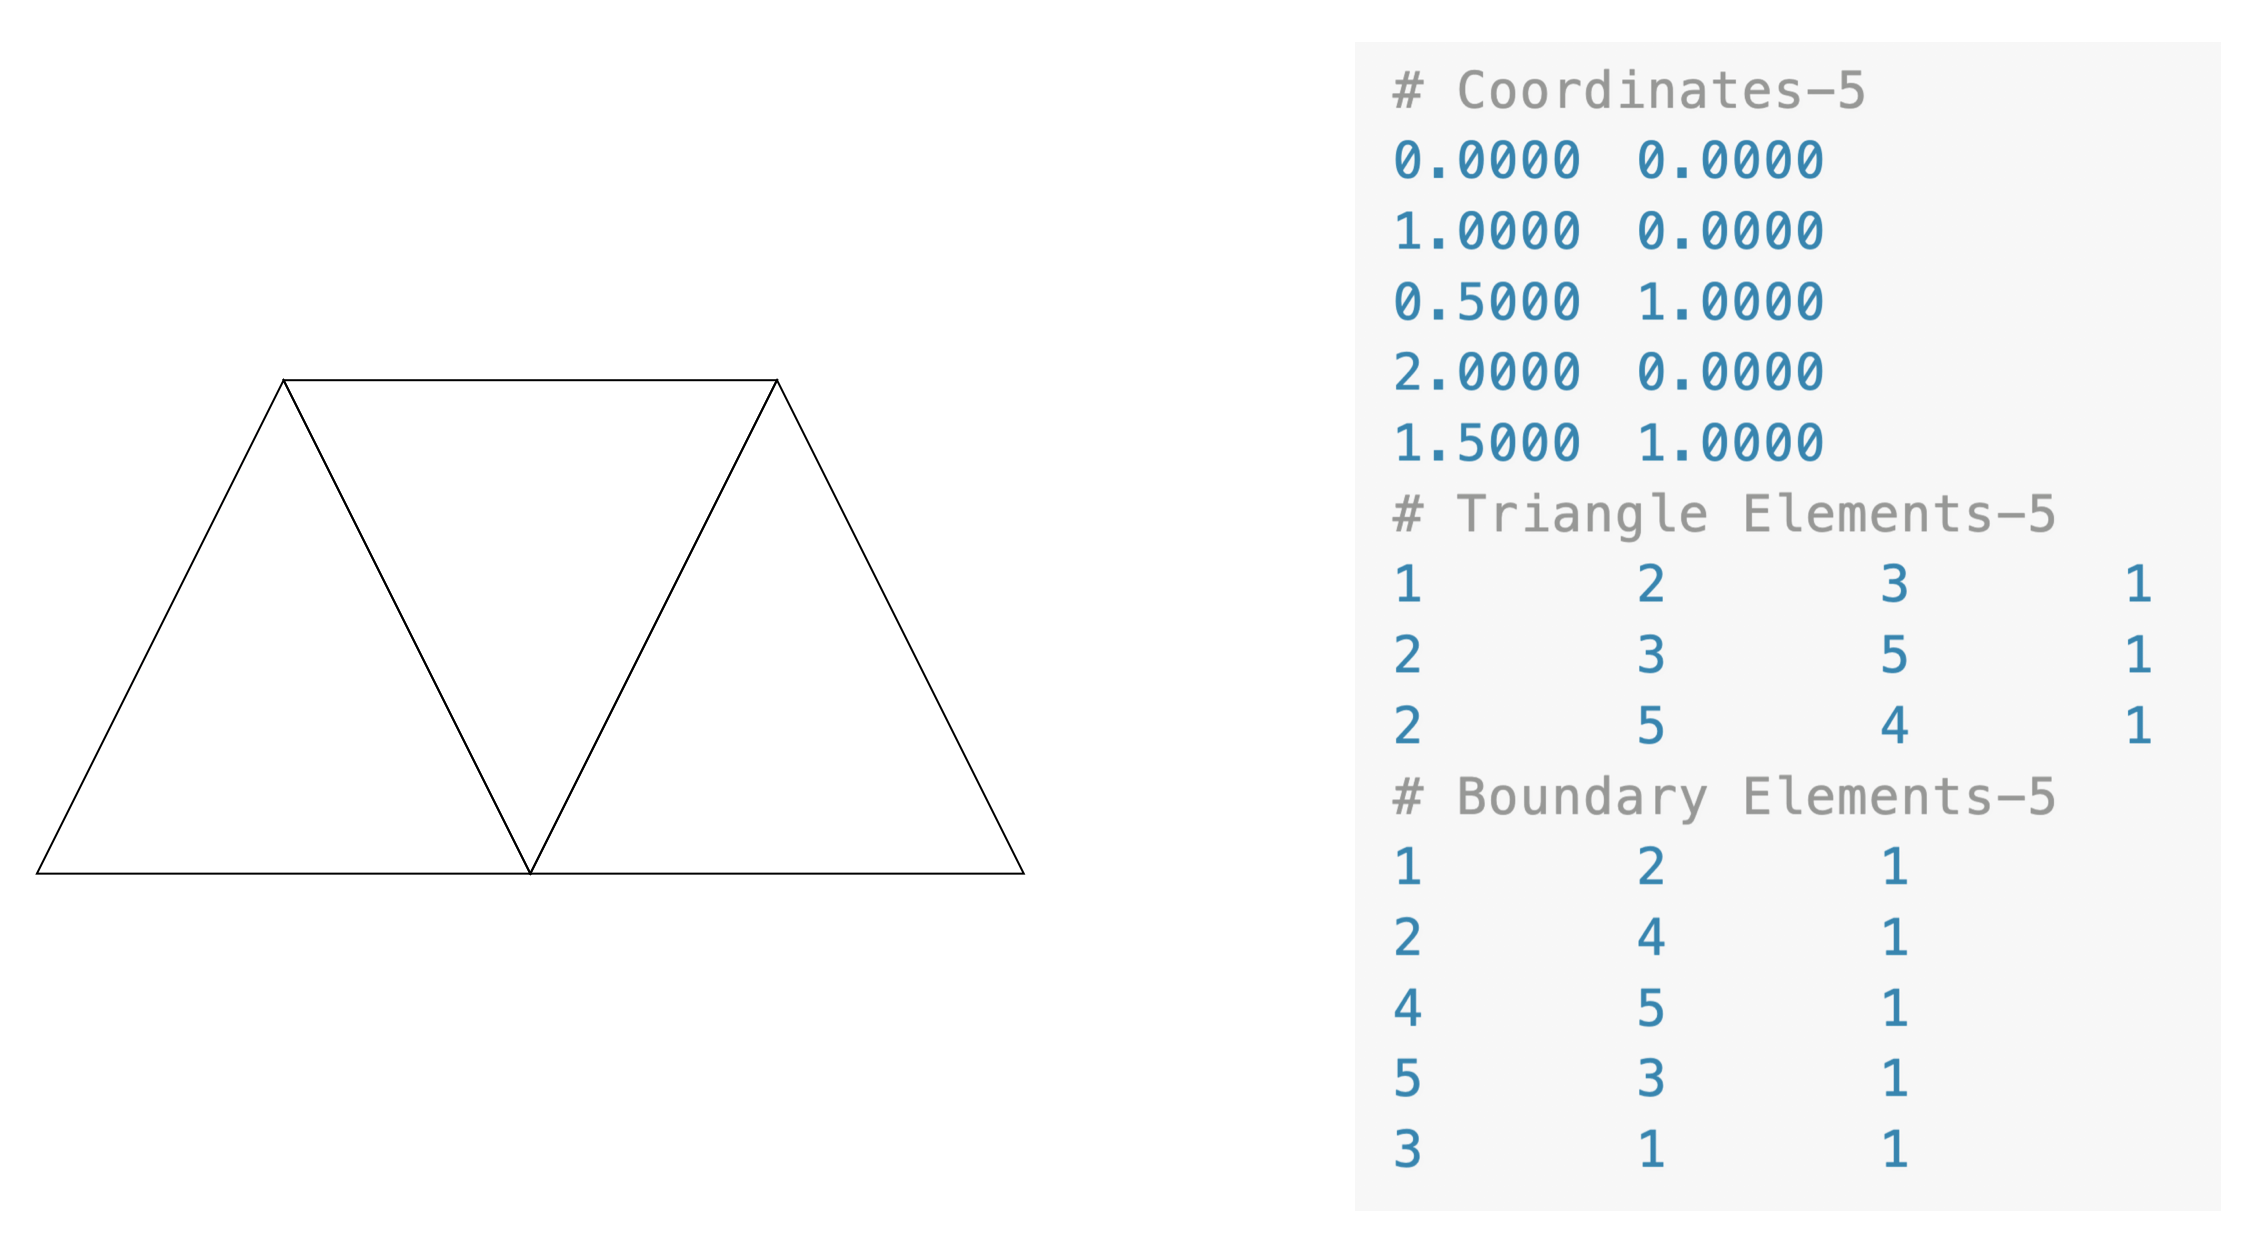
\includegraphics[width=3.5in]{meshdemo.png}
        \end{figure}
    \end{frame}
    \begin{frame}[fragile]\frametitle{Appendix: Matrix Assembly}

        Global stiffness matrix assembly code for reference
        {
        \small
        \begin{verbatim}
        [(element[i], element[j], shp_fn.stiffness_matrix[i, j]
        * alpha(marker)) for i in range(3) for j in range(3)
        for element, shp_fn, marker in
        zip(elements, shp_fns, markers)]
        \end{verbatim}
        }
        List of all (row, col, val) tuples, overlapping values are summed.
    \end{frame}
    
    \begin{frame}[fragile]\frametitle{Appendix: Gradient of $\alpha$}
        Given a function $\alpha(\|\nabla\phi\|)$ where
        \[\normm{\nabla\phi}=\normm{\left(\pdv{\vec{N}}{x}, \pdv{\vec{N}}{y} \right)^{\text{T}}\cdot \left(
        \begin{array}{c}
            \phi _i \\
            \phi _j \\
            \phi _k \\
        \end{array}
        \right)}\]
        \[\nabla\alpha=\frac{\alpha'(\normm{\nabla\phi})}{\normm{\nabla\phi}}
        \left(\pdv{\vec{N}}{x}\cdot\left(\pdv{\vec{N}}{x}\right)^{\text{T}}+
        \pdv{\vec{N}}{y}\cdot\left(\pdv{\vec{N}}{y}\right)^{\text{T}}\right)\cdot \left(
        \begin{array}{c}
            \phi _i \\
            \phi _j \\
            \phi _k \\
        \end{array}
        \right)\]
    \end{frame}
    \begin{frame}{Appendix: Torque Integration}
        First make a transformation to polar coordinates
        \[\left(
        \begin{array}{c}
            B_x(x,y) \\
            B_y(x,y) \\
        \end{array}
        \right) \to \left(
        \begin{array}{c}
            B_r(r,\theta) \\
            B_{\theta}(r,\theta) \\
        \end{array}
        \right) \]
        The vector $\left( B_r,\,B_{\theta} \right)^{\text{T}}$ is
        \[\left(
        \begin{array}{c}
            \cos (\theta )B_x(r \cos (\theta ),r \sin (\theta ))+\sin (\theta )B_y(r \cos (\theta ),r \sin (\theta )) \\
            \cos (\theta )B_y(r \cos (\theta ),r \sin (\theta ))-\sin (\theta )B_x(r \cos (\theta ),r \sin (\theta )) \\
        \end{array}
        \right)\]
        Torque per unit length is
        \[
            \frac{1}{\mu_0 (r_s-r_r)}\int_{r_r}^{r_s}\int_{0}^{2\pi} r^{2}B_r B_{\theta}\mathrm{d}\theta\mathrm{d}r
        \]
        This integral is easily approximated by sampling
    \end{frame}
\end{document}
